%%%%%%%%%%%%%%%%%%%%%%%%%%%%%%%%%%%%%%%%
% datoteka diploma-vzorec.tex
%
% vzorčna datoteka za pisanje diplomskega dela v formatu LaTeX
% na UL Fakulteti za računalništvo in informatiko
%
% vkup spravil Gašper Fijavž, december 2010
% 
%
%
% verzija 12. februar 2014 (besedilo teme, seznam kratic, popravki Gašper Fijavž)
% verzija 10. marec 2014 (redakcijski popravki Zoran Bosnić)
% verzija 11. marec 2014 (redakcijski popravki Gašper Fijavž)
% verzija 15. april 2014 (pdf/a 1b compliance, not really - just claiming, Damjan Cvetan, Gašper Fijavž)
% verzija 23. april 2014 (privzeto cc licenca)
% verzija 16. september 2014 (odmiki strain od roba)
% verzija 28. oktober 2014 (odstranil vpisno številko)
% verija 5. februar 2015 (Literatura v kazalu, online literatura)
% verzija 25. september 2015 (angl. naslov v izjavi o avtorstvu)
% verzija 26. februar 2016 (UL izjava o avtorstvu)
% verzija 16. april 2016 (odstranjena izjava o avtorstvu)
% verzija 5. junij 2016 (Franc Solina dodal vrstice, ki jih je označil s svojim imenom)


\documentclass[a4paper, 12pt]{book}
%\documentclass[a4paper, 12pt, draft]{book}  Nalogo preverite tudi z opcijo draft, ki vam bo pokazala, katere vrstice so predolge!



\usepackage[utf8x]{inputenc}   % omogoča uporabo slovenskih črk kodiranih v formatu UTF-8
\usepackage[slovene,english]{babel}    % naloži, med drugim, slovenske delilne vzorce
\usepackage[pdftex]{graphicx}  % omogoča vlaganje slik različnih formatov
\usepackage{fancyhdr}          % poskrbi, na primer, za glave strani
\usepackage{amssymb}           % dodatni simboli
\usepackage{amsmath}           % eqref, npr.
%\usepackage{hyperxmp}
\usepackage[hyphens]{url}  % dodal Solina
\usepackage{comment}       % dodal Solina

\usepackage[pdftex, colorlinks=true,
						citecolor=black, filecolor=black, 
						linkcolor=black, urlcolor=black,
						pagebackref=false, 
						pdfproducer={LaTeX}, pdfcreator={LaTeX}, hidelinks]{hyperref}

\usepackage{color}       % dodal Solina
\usepackage{soul}       % dodal Solina
\usepackage{listings}	% dodal Hrovat
\usepackage{float}		% dodal Hrovat

%%%%%%%%%%%%%%%%%%%%%%%%%%%%%%%%%%%%%%%%
%	DIPLOMA INFO
%%%%%%%%%%%%%%%%%%%%%%%%%%%%%%%%%%%%%%%%
\newcommand{\ttitle}{Mikrostoritve v decentraliziranem okolju}
\newcommand{\ttitleEn}{Microservices in decentralized environment}
\newcommand{\tsubject}{\ttitle}
\newcommand{\tsubjectEn}{\ttitleEn}
\newcommand{\tauthor}{Primož Hrovat}
\newcommand{\tkeywords}{decentralizacija, mikrostoritve, tehnologija veriženja podatkovnih blokov}
\newcommand{\tkeywordsEn}{decentralization, microservices, blockchain}


%%%%%%%%%%%%%%%%%%%%%%%%%%%%%%%%%%%%%%%%
%	HYPERREF SETUP
%%%%%%%%%%%%%%%%%%%%%%%%%%%%%%%%%%%%%%%%
\hypersetup{pdftitle={\ttitle}}
\hypersetup{pdfsubject=\ttitleEn}
\hypersetup{pdfauthor={\tauthor, ph0672@student.uni-lj.si}}
\hypersetup{pdfkeywords=\tkeywordsEn}


 


%%%%%%%%%%%%%%%%%%%%%%%%%%%%%%%%%%%%%%%%
% postavitev strani
%%%%%%%%%%%%%%%%%%%%%%%%%%%%%%%%%%%%%%%%  

\addtolength{\marginparwidth}{-20pt} % robovi za tisk
\addtolength{\oddsidemargin}{40pt}
\addtolength{\evensidemargin}{-40pt}

\renewcommand{\baselinestretch}{1.3} % ustrezen razmik med vrsticami
\setlength{\headheight}{15pt}        % potreben prostor na vrhu
\renewcommand{\chaptermark}[1]%
{\markboth{\MakeUppercase{\thechapter.\ #1}}{}} \renewcommand{\sectionmark}[1]%
{\markright{\MakeUppercase{\thesection.\ #1}}} \renewcommand{\headrulewidth}{0.5pt} \renewcommand{\footrulewidth}{0pt}
\fancyhf{}
\fancyhead[LE,RO]{\sl \thepage} 
%\fancyhead[LO]{\sl \rightmark} \fancyhead[RE]{\sl \leftmark}
\fancyhead[RE]{\sc \tauthor}              % dodal Solina
\fancyhead[LO]{\sc Diplomska naloga}     % dodal Solina


\newcommand{\BibTeX}{{\sc Bib}\TeX}

%%%%%%%%%%%%%%%%%%%%%%%%%%%%%%%%%%%%%%%%
% naslovi
%%%%%%%%%%%%%%%%%%%%%%%%%%%%%%%%%%%%%%%%  


\newcommand{\autfont}{\Large}
\newcommand{\titfont}{\LARGE\bf}
\newcommand{\clearemptydoublepage}{\newpage{\pagestyle{empty}\cleardoublepage}}
\setcounter{tocdepth}{1}	      % globina kazala

%%%%%%%%%%%%%%%%%%%%%%%%%%%%%%%%%%%%%%%%
% konstrukti
%%%%%%%%%%%%%%%%%%%%%%%%%%%%%%%%%%%%%%%%  
\newtheorem{izrek}{Izrek}[chapter]
\newtheorem{trditev}{Trditev}[izrek]
\newenvironment{dokaz}{\emph{Dokaz.}\ }{\hspace{\fill}{$\Box$}}

%%%%%%%%%%%%%%%%%%%%%%%%%%%%%%%%%%%%%%%%%%%%%%%%%%%%%%%%%%%%%%%%%%%%%%%%%%%%%%%
%% PDF-A
%%%%%%%%%%%%%%%%%%%%%%%%%%%%%%%%%%%%%%%%%%%%%%%%%%%%%%%%%%%%%%%%%%%%%%%%%%%%%%%


%%%%%%%%%%%%%%%%%%%%%%%%%%%%%%%%%%%%%%%% 
% define medatata
%%%%%%%%%%%%%%%%%%%%%%%%%%%%%%%%%%%%%%%% 
\def\Title{\ttitle}
\def\Author{\tauthor, ph0672@student.uni-lj.si}
\def\Subject{\ttitleEn}
\def\Keywords{\tkeywordsEn}

%%%%%%%%%%%%%%%%%%%%%%%%%%%%%%%%%%%%%%%% 
% \convertDate converts D:20080419103507+02'00' to 2008-04-19T10:35:07+02:00
%%%%%%%%%%%%%%%%%%%%%%%%%%%%%%%%%%%%%%%% 
\def\convertDate{%
    \getYear
}

{\catcode`\D=12
 \gdef\getYear D:#1#2#3#4{\edef\xYear{#1#2#3#4}\getMonth}
}
\def\getMonth#1#2{\edef\xMonth{#1#2}\getDay}
\def\getDay#1#2{\edef\xDay{#1#2}\getHour}
\def\getHour#1#2{\edef\xHour{#1#2}\getMin}
\def\getMin#1#2{\edef\xMin{#1#2}\getSec}
\def\getSec#1#2{\edef\xSec{#1#2}\getTZh}
\def\getTZh +#1#2{\edef\xTZh{#1#2}\getTZm}
\def\getTZm '#1#2'{%
    \edef\xTZm{#1#2}%
    \edef\convDate{\xYear-\xMonth-\xDay T\xHour:\xMin:\xSec+\xTZh:\xTZm}%
}

\expandafter\convertDate\pdfcreationdate 

%%%%%%%%%%%%%%%%%%%%%%%%%%%%%%%%%%%%%%%%
% get pdftex version string
%%%%%%%%%%%%%%%%%%%%%%%%%%%%%%%%%%%%%%%% 
\newcount\countA
\countA=\pdftexversion
\advance \countA by -100
\def\pdftexVersionStr{pdfTeX-1.\the\countA.\pdftexrevision}


%%%%%%%%%%%%%%%%%%%%%%%%%%%%%%%%%%%%%%%%
% XMP data
%%%%%%%%%%%%%%%%%%%%%%%%%%%%%%%%%%%%%%%%  
\usepackage{xmpincl}
\includexmp{pdfa-1b}

%%%%%%%%%%%%%%%%%%%%%%%%%%%%%%%%%%%%%%%%
% pdfInfo
%%%%%%%%%%%%%%%%%%%%%%%%%%%%%%%%%%%%%%%%  
\pdfinfo{%
    /Title    (\ttitle)
    /Author   (\tauthor, damjan@cvetan.si)
    /Subject  (\ttitleEn)
    /Keywords (\tkeywordsEn)
    /ModDate  (\pdfcreationdate)
    /Trapped  /False
}


%%%%%%%%%%%%%%%%%%%%%%%%%%%%%%%%%%%%%%%%%%%%%%%%%%%%%%%%%%%%%%%%%%%%%%%%%%%%%%%
%%%%%%%%%%%%%%%%%%%%%%%%%%%%%%%%%%%%%%%%%%%%%%%%%%%%%%%%%%%%%%%%%%%%%%%%%%%%%%%

\begin{document}
\selectlanguage{slovene}
\frontmatter
\setcounter{page}{1} %
\renewcommand{\thepage}{}       % preprecimo težave s številkami strani v kazalu
\newcommand{\sn}[1]{"`#1"'}                    % dodal Solina (slovenski narekovaji)
\renewcommand{\lstlistingname}{Izsek}

%%%%%%%%%%%%%%%%%%%%%%%%%%%%%%%%%%%%%%%%
%naslovnica
 \thispagestyle{empty}%
   \begin{center}
    {\large\sc Univerza v Ljubljani\\%
      Fakulteta za računalništvo in informatiko}%
    \vskip 10em%
    {\autfont \tauthor\par}%
    {\titfont \ttitle \par}%
    {\vskip 3em \textsc{DIPLOMSKO DELO\\[5mm]         % dodal Solina za ostale študijske programe
%    VISOKOŠOLSKI STROKOVNI ŠTUDIJSKI PROGRAM\\ PRVE STOPNJE\\ RAČUNALNIŠTVO IN INFORMATIKA}\par}%
    UNIVERZITETNI  ŠTUDIJSKI PROGRAM\\ PRVE STOPNJE\\ RAČUNALNIŠTVO IN INFORMATIKA}\par}%
%    INTERDISCIPLINARNI UNIVERZITETNI\\ ŠTUDIJSKI PROGRAM PRVE STOPNJE\\ RAČUNALNIŠTVO IN MATEMATIKA}\par}%
%    INTERDISCIPLINARNI UNIVERZITETNI\\ ŠTUDIJSKI PROGRAM PRVE STOPNJE\\ UPRAVNA INFORMATIKA}\par}%
%    INTERDISCIPLINARNI UNIVERZITETNI\\ ŠTUDIJSKI PROGRAM PRVE STOPNJE\\ MULTIMEDIJA}\par}%
    \vfill\null%
    {\large \textsc{Mentor}: prof.  dr.  Matjaž Branko Jurič\par}%
  % {\large \textsc{Somentor}:  izr.\ prof.\ dr. Martin Krpan \par}%
    {\vskip 2em \large Ljubljana, 2018 \par}%
\end{center}
% prazna stran
%\clearemptydoublepage      % dodal Solina (izjava o licencah itd. se izpiše na hrbtni strani naslovnice)

%%%%%%%%%%%%%%%%%%%%%%%%%%%%%%%%%%%%%%%%
%copyright stran
\thispagestyle{empty}
\vspace*{8cm}

\noindent
{\sc Copyright}. 
Rezultati diplomske naloge so intelektualna lastnina avtorja in Fakultete za računalništvo in informatiko Univerze v Ljubljani.
Za objavo in koriščenje rezultatov diplomske naloge je potrebno pisno privoljenje avtorja, Fakultete za računalništvo in informatiko ter mentorja.

\begin{center}
\mbox{}\vfill
\emph{Besedilo je oblikovano z urejevalnikom besedil \LaTeX.}
\end{center}
% prazna stran
\clearemptydoublepage

%%%%%%%%%%%%%%%%%%%%%%%%%%%%%%%%%%%%%%%%
% stran 3 med uvodnimi listi
\thispagestyle{empty}
\vspace*{4cm}

\noindent
Fakulteta za računalništvo in informatiko izdaja naslednjo nalogo:
\medskip
\begin{tabbing}
\hspace{32mm}\= \hspace{6cm} \= \kill




Tematika naloge:
\end{tabbing}
Opišite ključne arhitekturne koncepte in vzorce mikrostoritev ter proučite tehnologijo veriženja podatkovnih blokov. Identificirajte cilje in izzive decentraliziranega izvajanja mikrostoritev, kot nadgradnje obstoječih decentraliziranih konceptov. Pripravite arhitekturno zasnovo in implementirajte pilotno rešitev, ki bo demonstrirala možnosti izvajanja mikrostoritev na platformi Ethereum. Evalvirajte rešitev in identificirajte prednosti in pomanjkljivosti ter predlagajte možne izboljšave v prihodnosti. 
\vspace{15mm}



\vspace{2cm}

% prazna stran
\clearemptydoublepage

% zahvala
\thispagestyle{empty}\mbox{}\vfill\null\it%
\noindent
Zahvaljujem se prof. Matjažu B. Juriču za podporo in usmeritve pri pripravi diplomskega dela. Hvala članom Laboratorija za integracijo informacijskih sistemov za pomoč. Posebna zahvala pa gre mojim staršem, bratoma, sestrama, starim staršem in prijateljem, ki mi vedno stojijo ob strani in me pri mojem delu podpirajo.
\rm\normalfont

% prazna stran
\clearemptydoublepage

%%%%%%%%%%%%%%%%%%%%%%%%%%%%%%%%%%%%%%%%
% posvetilo, če sama zahvala ne zadošča :-)
% \thispagestyle{empty}\mbox{}{\vskip0.20\textheight}\mbox{}\hfill\begin{minipage}{0.55\textwidth}%
% Posvetilo
% \normalfont\end{minipage}

% prazna stran
\clearemptydoublepage


%%%%%%%%%%%%%%%%%%%%%%%%%%%%%%%%%%%%%%%%
% kazalo
\pagestyle{empty}
\def\thepage{}% preprecimo tezave s stevilkami strani v kazalu
\tableofcontents{}


% prazna stran
\clearemptydoublepage

%%%%%%%%%%%%%%%%%%%%%%%%%%%%%%%%%%%%%%%%
% seznam kratic

\chapter*{Seznam uporabljenih kratic}  % spremenil Solina, da predolge vrstice ne gredo preko desnega roba

\begin{comment}
\begin{tabular}{l|l|l}
  {\bf kratica} & {\bf angleško} & {\bf slovensko} \\ \hline
  % after \\: \hline or \cline{col1-col2} \cline{col3-col4} ...
  {\bf CA} & classification accuracy & klasifikacijska točnost \\
  {\bf DBMS} & database management system & sistem za upravljanje podatkovnih baz \\
  {\bf SVM} & support vector machine & metoda podpornih vektorjev \\
\end{tabular}
\end{comment}

\noindent\begin{tabular}{p{0.1\textwidth}|p{.4\textwidth}|p{.4\textwidth}}    % po potrebi razširi prvo kolono tabele na račun drugih dveh!
  {\bf kratica} & {\bf angleško}                             & {\bf slovensko} \\ \hline
  {\bf API}      & application programming interface & aplikacijski programski vmesnik \\
  {\bf PoW} & Proof-of-Work & dokaz o opravljenem delu \\
  {\bf DBMS}   & Database Management System & sistem za upravljanje podatkovne baze \\
  {\bf IPFS} & Interplanetary File System & medplanetarni datotečni sistem \\
  {\bf REST} & Representational state transfer & Reprezentativni prenos stanja \\
  {\bf GKE} & Google Kubernetes Engine & Google Kubernetes Engine \\
  {\bf AWS} & Amazon Web Services & Amazon Web Services \\
  {\bf DOS} & Denial of Service & zavrnitev storitve \\
  {\bf CNCF} & Cloud Native Computing Foundation & Fundacija za oblačno računalništvo \\
\end{tabular}


% prazna stran
\clearemptydoublepage

%%%%%%%%%%%%%%%%%%%%%%%%%%%%%%%%%%%%%%%%
% povzetek
\addcontentsline{toc}{chapter}{Povzetek}
\chapter*{Povzetek}

\noindent\textbf{Naslov:} \ttitle
\bigskip

\noindent\textbf{Avtor:} \tauthor
\bigskip

%\noindent\textbf{Povzetek:} 
\noindent

Mikrostoritve danes vztrajno prevzemajo primat v svetu razvoja programske opreme kjer nadomeščajo tradicionalne aplikacije. 
Način gradnje omogoča učinkovitejše skaliranje, distribuiranje in medsebojno odkrivanje.
Aplikacije, grajene v arhitekturi mikrostoritev se večinoma izvajajo v ra\-ču\-nal\-ni\-ških oblakih.
Učinkovitejše skaliranje in elastičnost mikrostoritvam omogoča ohranjati dobre performančne lastnosti in odgovoriti na tisoče so\-časnih zahtevkov.
Danes mikrostoritve za izvajanje zahtevajo centralizirano okolje strežnikov, skupaj s tehnologijo vsebnikov.
V diplomski nalogi smo raziskali področje decentraliziranega izvajanja mikrostoritev in razvili prototip, ki demonstrira izvajanje mikrostoritev na platformi Ethereum.
Zamišljamo si sistem, v katerem ne poznamo izpadov storitev ter dolgih odzivnih časov.
V nalogi smo se osredotočili na decentralizirano odkrivanje storitev ter razvili prvi prototip aplikacije in razširitve za ogrodje KumuluzEE, ki demonstrirata decentraliziran način izvajanja.
Gre za pomembno svetovno novost, ki ima potencial začrtati nove smernice v računalniški panogi.

\bigskip

\noindent\textbf{Ključne besede:} \tkeywords.
% prazna stran
\clearemptydoublepage

%%%%%%%%%%%%%%%%%%%%%%%%%%%%%%%%%%%%%%%%
% abstract
\selectlanguage{english}
\addcontentsline{toc}{chapter}{Abstract}
\chapter*{Abstract}

\noindent\textbf{Title:} \ttitleEn
\bigskip

\noindent\textbf{Author:} \tauthor
\bigskip

%\noindent\textbf{Abstract:} 
\noindent 

Today microservices are one of the leading design principles, when it comes to building modern applications.
Monoliths are being replaced with this modern architecural style and multiple tools and techniques are being develop to support it.
Applications are deployed to a computing center, often called simply as cloud.
Elasticity and effective scaling of such applications in contrast to monoliths are needed for good performance and high response rates.
We have analized the subjet of a decentralized execution and implemented a prototype platform based on Ethereum blockchain.
We have proposed a conceptual solution to service discovery in a decentralized environment and presented a process, that enables decentralized execution of applications.
We are standing on the edge of what we know is currently possible and are ready to push the boundaries even further. This can be the next big step in computer science.

\bigskip

\noindent\textbf{Keywords:} \tkeywordsEn.
\selectlanguage{slovene}
% prazna stran
\clearemptydoublepage

%%%%%%%%%%%%%%%%%%%%%%%%%%%%%%%%%%%%%%%%
\mainmatter
\setcounter{page}{1}
\pagestyle{fancy}

\chapter{Uvod}
Poslovne storitve se danes selijo v oblak.
S pojavom arhitekture mikrostoritev in tehnologije vsebnikov ter orodij za njihovo orkestracijo, so nekdaj monolitne aplikacije  pričele razpadati na manjše, logično ločene sestavne dele.
Razmeroma majhne in neodvisne aplikacije, specializirane za opravljanje točno določenih nalog, omogočajo hiter vzpostavitveni čas in so razmeroma performančno manj zahtevne.
Neodvisnost teh aplikacij nam omogoča tudi skaliranje posameznih delov celotne storitve, ko je to potrebno.

Vsebniki so razmeroma stara tehnologija, ki je s pojavom okolja Docker doživela pravi razcvet.
Gre za t. i. lahko virtualizacijo, ki poteka na nivoju procesov in ne na nivoju operacijskega sistema.
Pravi potencial vsebnikov izkoristimo z uporabo orkestratorjev kot so Kubernetes, Amazon ECS, Google Kubernetes Engine (GKE), Docker Swarm, Azure Container Service in podobni.
Ta orodja omogočajo spremljanje, zaganjanje, zaustavljanje in preverjanje storitev skladno z uporabniško podanimi zahtevami.
Storitve se izvajajo distribuirano (porazdeljeno) in replicirano, pogosto na fizično ločenih sistemih, kar zagotavlja visoko stopnjo odzivnosti in dosegljivosti. Razpoložljivost in dosegljivost storitev se danes meri predvsem na peti ali šesti decimalki, t. i. \sn{število devetic} (ang. number of nines).

Pred desetimi leti se je s pojavom digitalne valute Bitcoin pričel hiter razvoj decentralizirane tehnologije, ki omogoča nespremenljivo in preverljivo hrambo podatkov na poljubnih napravah v omrežju \cite{nakamoto2008bitcoin}.
Tehnologija, poznana pod imenom veriženje podatkovnih blokov (ang. blockchain), je hitro povezala računalniške zanesenjake ter povzročila ustanovitev različnih fundacij, ki se ukvarjajo z njenim razvojem.
Med bolj znanimi sta fundaciji Hyperledger in Ethereum \cite{hyperledgerWeb, ethereumweb}.

Sistemi za izvajanje mikrostoritev so replicirani in distribuirani, vendar ne decentralizirani.
Za arhitekturo, ki podpira izvajanje naših storitev, skrbi ena, centralna identiteta, najsi bo to Google, Amazon, Microsoft ali pa zasebni oblak oz. izvajalno okolje.
Glavni cilj te diplomske naloge je aplicirati koncepte decentralizirane shrambe podatkov na nivo poslovne logike.
Povezati želimo tehnologijo podatkovnih blokov in arhitekturo mikrostoritev na način, da zagotovimo večjo decentralizirano izvajanje. 
Na osnovi tega želimo doseči večjo robustnost in odpornost celotnega sistema ter visoko razpoložljivost.
V diplomski nalogi smo razvili prototip rešitve za decentralizirano izvajanje mikrostoritev.
Sistem sestavlja poljubno mnogo med seboj povezanih entitet.
Entiteta je naprava, ki izvaja protokol za decentralizirano izvajanje storitev.
Te so pripravljene proti plačilu izvajati storitve na željo naročnika.
Sodelovanje v omrežju je brezplačno in dostopno vsakomur, za opravljeno delo pa izvajalec prejme vnaprej predpisano nagrado.
Celoten sistem sestoji iz množice različnih komponent, ki skupaj zagotavljajo preverljivost pravilnosti izvedenih operacij ter učinkovito porazdeljevanje ter prerazporejanje dela med entitetami.
Naloga ene izmed osrednjih komponent je zagotoviti učinkovito odkrivanje trenutno aktivnih storitev.
Zasnova in razvoj te komponente je osrednji del te diplomske naloge, pred tem pa so predstavljene uporabljene tehnologije in tehnike.

\chapter{Arhitekturni koncepti mikrostoritev}
\label{ch1}

Razvoj monolitnih aplikacij je dobro razumljiv in podprt v vseh danes prisotnih razvojnih okoljih.
Celotna poslovna logika aplikacije je zbrana na enem mestu ter razdeljena po modulih, ki komunicirajo prek programskih klicev.
Aplikacija vključuje tudi vse potrebne odvisnosti za delovanje (knjižnice, razširitve...).
Prenos in namestitev teh storitev na strežniške sisteme je enostaven postopek, rešitev v obliki izvršljivih datotek ali s kopiranjem direktorijske strukture prenesemo v produkcijsko izvajalno okolje.
Različni sestavni deli aplikacije so med seboj močno sklopljeni (medprocesna komunikacija), za uveljavitev sprememb enega dela sistema je potrebno celotno aplikacijo ponovno namestiti.
Življenjski cikel takih aplikacij je po navadi dolg, sklopljenost sistema namreč ne omogoča enostavne menjave sestavnih delov ali celo programskega okolja.

Arhitektura mikrostoritev rešuje nekatere probleme monolitnih aplikacij, na račun večje kompleksnosti celotnega sistema.
Šibka sklopljenost sestavnih delov je glavna prednost arhitekture, komunikacija med njimi pa običajno poteka preko lahkih omrežnih tehnologij (HTTP) ali asinhronih sporočilnih sistemov (sporočilne vrste, dogodkovno gnani sistemi).
Arhitektura nam omogoča enostavnejšo menjavo sestavnih delov aplikacije, kar privede do krajšega življenjskega cikla in uvedbe praks sprotne dostave in sprotne integracije \cite{monolithMicroservice}.


\section{Arhitektura mikrostoritev}

Gradnja aplikacij je do nedavnega potekala na način, da so razvijalci vse odvisnosti in programsko logiko, potrebno za delovanje, zložili skupaj v veliko tvorbo -- monolit.
Tak način gradnje ima svoje prednosti in slabosti.
Prednosti na eni strani predstavljajo enostavnejša zgradba aplikacije, celotna izvorna koda projekta se prevede v eno storitev.
Orodja za razvoj so prilagojena takšnemu načinu dela in razvijalcu ponujajo širok nabor funkcij, ki podpirajo celotno življenjsko pot aplikacije; od razvoja, testiranja, namestitve v testna in produkcijska okolja ter vzdrževanja.
Velikost projekta je na drugi strani ena od slabosti monolitov, majhne spremembe enega sestavnega dela potrebujejo ponovno namestitev celotne aplikacije.
Skaliranje poteka vertikalno, preko ustvarjanja novih instanc celotne aplikacije.
Monolitna zasnova aplikacije razvijalce in vzdrževalce zaveže k dolgoročni uporabi tehnologij, ki so bile uporabljene na začetku.
Kasnejše uveljavljanje novih tehnologij oziroma nadomeščanje obstoječih je časovno in finančno potratno, celotno logiko aplikacije je potrebno prepisovati \cite{monolithMicroservice}.

Arhitektura mikrostoritev se problema gradnje aplikacij loti drugače.
Aplikacijo se logično razbije na posamezne sestavne dele, ki se izvajajo samostojno in se med seboj povezujejo preko lahkih komunikacijskih protokolov (malo režijskih podatkov pri prenosu sporočil) ali asinhronih sporočilnih sistemov.
Vsak sestavni del aplikacije je samostojen v smislu skaliranja, življenjske dobe posamezne instance, razvoja in podpornih tehnologij \cite{7030212}.
Tak način gradnje sledi vzoru, ki ga v fizičnem svetu poznamo že stoletja, to je sestavljanje vnaprej pripravljenih delov v celoto.
Lep primer tega je avtomobilska industrija.
Na tekočem traku se na tisoče sestavnih delov različnih proizvajalcev zloži v polno funkcionalno enoto -- avtomobil.
Podobno želimo doseči pri razvoju programske opreme, kar bi pohitrilo in pocenilo razvoj novih aplikacij, krepko pa bi omejili tudi nepotrebno podvajanje izvorne kode \cite{microservicePattern, microservicesMartin}.

V povezavi z mikrostoritvami je tesno povezana tudi arhitektura \textit{cloud-native}.
Gre za novo paradigmo razvoja programske opreme.
Z namenom uveljavljanja in razvoja paradigme je bila ustanovljena \textit{Cloud Native Computing Foundation (CNCF)}, ki bdi nad razvojem standardov in novih smernic.
Oblačne sisteme tako po definiciji fundacije sestavljajo \cite{cncf}:
\begin{itemize}
	\item Aplikacije in procesi, ki se izvajajo znotraj vsebnikov. Vsebniki so neodvisne in izolirane izvajalne enote.
	\item Storitve, ki se dinamično upravljajo in nadzorujejo preko centralnega orkestracijskega procesa.
	\item Mikrostoritve, ki so sestavni deli sistema in so med seboj šibko sklopljene.
\end{itemize}

Računalništvo v oblaku je uporaba in dostop do računskih virov (aplikacije, podatkovna skladišča, procesorski čas...) na zahtevo preko interneta.
Plačilo se izvede skladno s količino porabljenih virov.
Viri so elastični in zmožni hitrega in učinkovitega skaliranja ter prilagajanja trenutnim zahtevam.
V grobem med seboj ločimo tri glavne tipe oblačnih sistemov: SaaS, PaaS in IaaS \cite{ibmCloudComputing}.
SaaS (ang. Software as a Service) -- programska oprema kot storitev, je oblačna aplikacija, ki se izvaja na oddaljenih računalnikih, do katerih uporabnik storitve dostopa preko interneta. 
Prednosti teh aplikacij so dostopnost od koderkoli, za nemoteno delovanje aplikacije je odgovoren ponudnik.
Storitev je zmožna dinamičnega skaliranja, da zadovolji trenutnim potrebam.
PaaS (ang. Platform as a Service) -- platforma kot storitev, uporabnikom ponuja programsko platformo, brez stroškov nakupa in kompleksnosti upravljanja podporne strojne in programske opreme.
IaaS (ang. Infrastructure as a Service) -- infrastruktura kot storitev, ponuja dostop do računskih virov (strežniki, omrežna oprema, shramba...).
Uporabnikom ni potrebno investirati v lastno strojno opremo, podobno kot obe sestrski storitvi (SaaS in PaaS), je tudi ta zmožna samodejnega skaliranja \cite{ibmCloudComputing, TOFFETTI2017165}.

Za razvoj spletnih aplikacij (SaaS) se je pojavila dodatna metodologija, poznana pod imenom The Twelve-Factor App.
Metodologija predpisuje dobre prakse za razvoj aplikacij, z možnostjo učinkovitega skaliranja, menjave okolij, avtomatizacije gradnje ter namestitve in zmanjševanjem razlik med produkcijskim in razvojnim okoljem.
Metodologija zajema naslednje faktorje \cite{12factor}:
\begin{itemize}
	\item en sistem za upravljanje z verzijami
	\item odvisnosti so eksplicitno navedene in izolirane
	\item konfiguracija je shranjena v okolju
	\item podporne storitve se uporabljajo kot viri
	\item strogo ločene faze gradnje in izvajanja storitve
	\item aplikacije se izvajajo kot en ali več med seboj neodvisnih procesov
	\item aplikacije so dostopne preko omrežnih vrat
	\item skaliranje aplikacij na osnovi posameznih procesov
	\item hitri zagonski časi ter sprostitev vseh odprtih povezav ob zaustavitvi
	\item razvojno, testno in produkcijsko okolje naj bodo med seboj čim bolj podobni
	\item dnevniški zapisi se obravnavajo kot niz dogodkov
	\item ločen administratorski proces
\end{itemize}

Dodatna prednost, ki jo prinaša arhitektura \sn{cloud-native}, je tudi hitrost razvoja samih aplikacij.
Delitev na manjše osnovne dele omogoča hiter razvoj novih funkcionalnosti, lažje testiranje in nadgradnje.
Z uporabo integracijskih orodij in tehnik zmanjšuje čas objave in zmanjša stroške vzdrževanja \cite{stine2015migrating}.


\section{Podporni mehanizmi za delovanje mikrostoritev}

Ključne lastnosti mikrostoritev so predvsem ozka usmerjenost v reševanje specifičnih problemov.
Storitve so med seboj šibko sklopljene, kar predstavlja prednost pri nadgradnjah in menjavi implementacije.
Za delovanje sistema, vsaj v teoriji, potrebujemo le jasno določene vmesnike.
Upravljanje in usklajevanje storitev prevzema centralna avtoriteta, vsaka storitev je sama odgovorna za svoje podatke.
Napake so v dinamičnem sistemu pogoste, njihovo učinkovito zaznavanje in upravljanje je v domeni tako nadzornika kot storitve same.
Celoten sistem lahko primerjamo z operacijskim sistemom Unix, ki ga sestavlja vrsta med seboj neodvisnih procesov, ki opravljajo ozko usmerjeno nalogo, med seboj pa jih povezujemo preko cevovodov.
Pri mikrostoritvah cevovode nadomestimo z omrežnimi protokoli (HTTP, gRPC) \cite{microservicesMartin}.

Vsaka storitev je samostojna in zadolžena za ustvarjanje lastnih dnevniških zapisov.
Za pregled nad vsemi dnevniškimi zapisi v celotnem sistemu se uporablja tehnika zbiranja zapisov na enem, centralnem, delu.
Razvite so tudi naprednejše tehnike zaznavanja in odpravljanja napak, ki so v velikih in kompleksnih sistemih vedno prisotne -- odpornost na napake.
Ena izmed tehnik pri reševanju napak je uporaba prekinjevalcev toka (ang. circuit breaker)\cite{sarcMag}.

Dodatno so v naslednjih podpoglavjih podrobneje predstavljeni še trije mehanizmi, značilni za arhitekturo mikrostoritev: spremljanje metrik, preverjanje vitalnosti ter odkrivanje storitev.
Ustrezno povezani v celoto predstavljajo skoraj vse elementarne dele sistema, sposobnega decentraliziranega izvajanja.
Za učinkovit sistem potrebujemo načine kako ugotoviti, katere storitve delujejo po pri\-ča\-ko\-va\-njih ter katera izmed sodelujočih entitet v omrežju nam lahko najhitreje ponudi odgovor na zahtevo -- izvede zahtevano storitev.

\subsection{Spremljanje metrik}

Posamezna mikrostoritev se lahko izvaja na različnih (fizičnih) lokacijah, na različni strojni opremi in v več instancah.
Pojavi se potreba po spremljanju storitve in njenega obnašanja, kje in zakaj prihaja do izpadov ter morebitnih dolgih odzivnih časih.
Vse želene metrike želimo shraniti na enem centralnem mestu, jih po možnosti agregirati, in tako omogočiti enostavno odkrivanje napak in njihovo reševanje.
V osnovi poznamo dva modela zbiranja metrik: 
\begin{itemize}
	\item mikrostoritev sama pošilja metrike centralni zbirki (ang. push)
	\item centralna zbirka zahteva metrike od storitve (ang. pull)
\end{itemize}

Zbiranje metrik ponuja dober vpogled v obnašanje posameznih mikrostoritev, s sabo pa prinese dodatno potrebno infrastrukturo in dodatne težave pri implementaciji \cite{ApplicationMetrics}.


Ena izmed bolj znanih storitev za zbiranje aplikacijsih metrik je Prometheus, odprtokodna zbirka orodij za zbiranje in agregiranje metrik ter obveščanje.
Projekt je bil kmalu za orkestracijskim okoljem Kubernetes pridružen fundaciji CNCF.
Prometheus metrike zahteva od storitve (način pull), jih agregira in ob tem proži morebitna opozorila.
Skupaj z ogrodjem Grafana omogoča celovit, tudi vizualni, vpogled v zbrane metrike \cite{Prometheus}.

\subsection{Preverjanje vitalnosti}

Pogosto se zgodi, da se mikrostoritev še vedno odziva na posamezne zahtevke, vendar ne deluje pravilno.
V takšnih primerih je pričakovano obnašanje sistema, da nedelujočo mikrostoritev označi kot nedosegljivo in jo nadomesti z novo.
Tu v igro vstopi koncept preverjanja vitalnosti storitev (ang. health check), ki za vsako mikrostoritev pričakuje izpostavljeno dostopno točko, preko katere sistem pridobi informacije o sposobnosti storitve, da pravilno odgovori na zahtevke.
Vsaka mikrostoritev je odgovorna za preverjanje svojih zunanjih in notranjih virov in generiranja poročila o trenutnem statusu posamezne komponente.
Tipični testi so preverjanje zmožnosti povezave na podatkovno bazo, dosegljivost ostalih odvisnih storitev, povezljivost z vrstami ipd.
Poleg zunanjih odvisnosti se preveri tudi stanje gostitelja: razpoložljiv prostor na disku, zasedenost CPE ipd.
Nadzorna storitev periodično proži zahteve na vse registrirane storitve in preverja njihove odzive.
Tipičen ukrep ob negativnem odzivu je zaustavitev in ponovni zagon nedelujoče storitve \cite{healthCheck}.

\subsection{Odkrivanje storitev}

Ko želimo od zunanje entitete pridobiti podatke oziroma prožiti določeno akcijo, potrebujemo njen omrežni naslov (kombinacija naslova IP in številke vrat).
Pri klasičnih aplikacijah, ki se izvajajo na fizičnih napravah, so naslovi relativno statični.
Zelo malo je tudi klicev med posameznimi aplikacijami, saj se storitve med seboj kličejo preko programskih klicev.
V arhitekturi mikrostoritev je omrežnih klicev bistveno več, ker je celotna programska logika aplikacije sestavljena iz več samostojnih storitev.
Njihovo število se dinamično spreminja, skladno s tem tudi omrežni naslovi posameznih instanc.
Posledično je potrebno za odjemalca vpeljati nov mehanizem, ki je zmožen dinamično odkriti naslove, na katerih se želena storitev nahaja.

Tipično za oblačne arhitekture je, da se odkrivanje storitev realizira s pomočjo centralnega registra.
Storitve se ob pričetku izvajanja registrirajo.
Odjemalna aplikacija ob potrebi po dostopu do zunanje storitve na register naslovi poizvedbo za lokacijo trenutno aktivnih instanc želene storitve.
Zakasnitev pri omrežnih klicih je bistveno večja kot pri programskih klicih znotraj aplikacije, zato želimo visoko učinkovitost poizvedb \cite{serviceDiscovery, maldip}.

\section{Vsebniki in orkestracija}

Vsebniki danes nadomeščajo virtualne naprave (ang. virtual machines), predvsem na račun bolj učinkovite uporabe sistemskih virov in odpravljanjem ne\-po\-tre\-bnih podvajanj nivojev programske opreme, predvsem na nivoju operacijskega sistema.

\subsection{Tehnologija vsebnikov}
Vsebnik je samostojen, izvršljiv skupek programske opreme, ki vsebuje vse potrebne odvisnosti, orodja, knjižnice in nastavitve, potrebne za izvajanje.
Izvajanje kode znotraj vsebnika je na vsakem gostiteljskem okolju (Windows, Linux, MacOS) enako.
Notranji deli vsebnika so izolirani od okolice, kar odpravlja morebitne konflikte zaradi različnih verzij potrebnih odvisnosti.
V primerjavi z virtualnimi napravami vsebniki virtualizirajo operacijski sistem in ne podporne strojne opreme.
Z gostiteljskim sistemom in ostalimi vsebniki delijo jedro operacijskega sistema, vsak izmed njih v svojem naslovnem prostoru.

Slika \ref{vm_vs_container} prikazuje bistveno razliko med vsebniško tehnologijo in tehnologijo virtualnih naprav \cite{dockerContainer}.

\begin{figure}[h]
	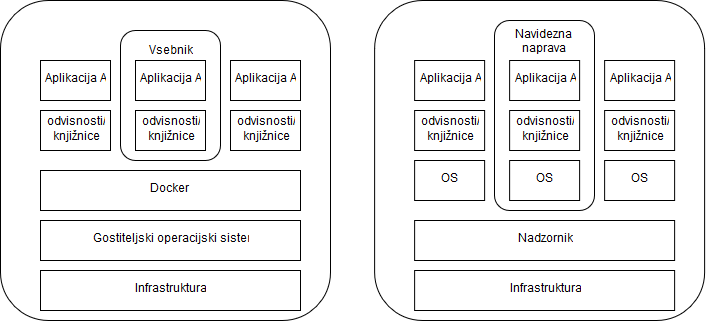
\includegraphics[width=1.0\textwidth]{slike/vsebniki_vm.png}
	\caption{Primerjava vsebnikov in virtualnih naprav.}
	\label{vm_vs_container}
\end{figure}


\subsection{Orkestracijska orodja}

Proces prenosa in namestitve vsebnikov v izvajalno okolje je moč avtomatizirati.
Proces postaja pomembnejši z rastjo števila vsebnikov in gostiteljskih sistemov. 
Ta tip avtomatizacije imenujemo orkestracija, ponuja pa nam vrsto funkcionalnosti \cite{mongoKubernetes}:
\begin{itemize}
	\item upravljanje z gostiteljskim sistemom
	\item instanciranje vsebnikov
	\item upravljanje z vsebniki
	\item povezovanje vsebnikov preko vmesnikov
	\item izpostavljanje storitev zunanjim napravam
	\item skaliranje gruče vsebnikov
\end{itemize}

S pojavom in razširitvijo vsebniške tehnologije so se pojavila tudi številna orodja za orkestracijo.
Med njimi sta najbolj poznana Docker Swarm in Kubernetes.
Vsako izmed naštetih orodij orkestracijo rešuje na svoj način, Kubernetes je trenutno eno izmed najbolj razširjenih orodij.
Njegove glavne funkcionalnosti so:
\begin{itemize}
	\item avtomatizirano nameščanje in repliciranje vsebnikov
	\item skaliranje
	\item porazdeljevanje dela (ang. load balancing)
	\item progresivno nameščanje posodobitev
	\item odpornost na napake in odpovedi vsebnikov s samodejnimi ponovnimi zagoni
	\item kontrolirano izpostavljanje notranjega omrežja zunanjim storitvam
\end{itemize}

Glavni sestavni deli Kubernetesa \cite{mongoKubernetes}: 
\begin{itemize}
	\item gruča (ang. cluster): zbirka enega ali več strežnikov (ang. node), ki svoje vire ponujajo nadzornemu procesu
	\item strok (ang. pod): skupina vsebnikov in pripadajočih shramb, ki so dodeljene enemu gostitelju. Predstavljajo osnovno enoto Kubernetesa, znotraj stroka si procesi delijo lokalni omrežni naslovni prostor.
	\item oznake (ang. labels): dodeljene oznake posameznim entitetam, ki omogočajo upravljanje z njimi v skupini
	\item storitve: skrbijo za osnovno dodeljevanje dela in izpostavljajo stroke zunanjemu svetu.
\end{itemize}

Slika \ref{kubernetes_cluster} prikazuje osnovno shemo Kubernetes gruče.

\begin{figure}[h]
	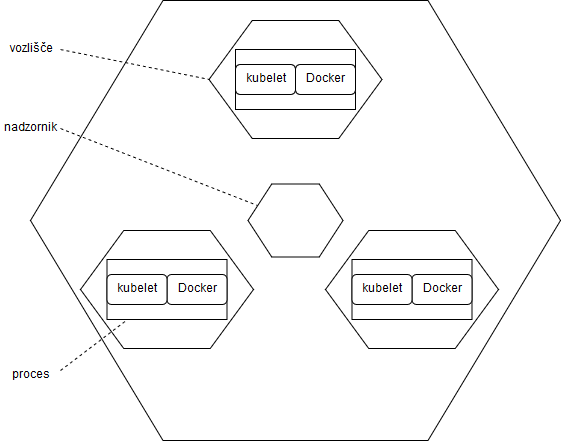
\includegraphics[width=1.0\textwidth]{slike/kubernetes_cluster.png}
	\caption{Kubernetes gruča \cite{kubernetesTutorial}.}
	\label{kubernetes_cluster}
\end{figure}

V tem poglavju smo pregledali arhitekturo mikrostoritev ter jo primerjali s klasično monolitno zasnovo aplikacij.
Opisali smo tipične vzorce in tehnike ter orodja, ki se uporabljajo pri tej arhitekturi.
V naslednjem poglavju bomo pregledali tehnologijo veriženja podatkovnih blokov, kar bo osnova za realizacijo glavnega cilja diplomske naloge -- arhitekture za decentralizirano izvajanje mikrostoritev.

\chapter{Tehnologija veriženja podatkovnih blokov in decentralizacija}
\label{ch2}

Tehnologija veriženja podatkovnih blokov je v svetu računalništva uveljavila koncept decentralizacije.
Pri decentralizaciji gre za skupek povezanih entitet, ki so med sabo neodvisne, med njimi je omogočena interakcija, vsaka med njimi pa hrani svojo lokalno kopijo trenutnega stanja omrežja.
Lokalno shranjeno stanje omrežja pri entiteti se mora ujemati z vsemi ostalimi stanji udeležencev v omrežju.
Udeleženec lahko stanje omrežja spreminja le v primeru, da se z želenimi spremembami strinja zadosten delež vseh udeležencev (običajno večina).
V kolikor temu ni tako, se spremembe ne shranijo oziroma se razveljavijo.

Izvajanje aplikacijske poslovne logike uvrščamo med nivo hrambe podatkov in nivo uporabniškega vmesnika.
Decentralizirano hrambo podatkov danes že poznamo, od tu pa gradimo in razmišljamo naprej, v smeri decentralizacije poslovne logike.
V tem poglavju bomo predstavili tehnologijo in osnovne ideje, ki omogočajo porazdeljeno hrambo podatkov.
Koncepti pri decentralizirani hrambi podatkov predstavljajo osnovo in odskočno desko za decentralizirano izvajanja poslovne logike.
Podatkovni bloki nam omogočajo trajno in nespremenljivo sklepanje ter zapis dogovorov o podrobnostih izvajanja, kar je nujno za zanesljiv sistem takšnih storitev.

Veriženje podatkovnih blokov je peer-to-peer porazdeljena podatkovna shramba, dosežena s soglasjem, sistemom pametnih pogodb ter drugih po\-mo\-žnih tehnologij \cite{hyperledgerWeb}. 
Osrednja komponenta sistema je glavna knjiga (ang. ledger), ki beleži vse akcije (transakcije), izvedene na omrežju \cite{hyperledgerDocs}.
Entiteta, ki transakcijo izvede, le-to podpiše s svojim privatnim ključem.
Skupek transakcij tvori podatkovni blok, bloki se med seboj povezujejo v podatkovno verigo.
Posamezne člene verige med seboj povezuje zgoščevalna funkcija, na vhod katere postavimo zgoščeno vrednost trenutnega in prejšnjega bloka.
Podatkovno verigo je moč vedno le podaljševati, trenutno veljavno in resnično stanje omrežja je trenutno najdaljša serija blokov.
Celotna veriga blokov je replicirana na vsaki sodelujoči entiteti.
Slika \ref{blockchain} shematsko prikazuje podatkovno verigo.

\begin{figure}[h]
	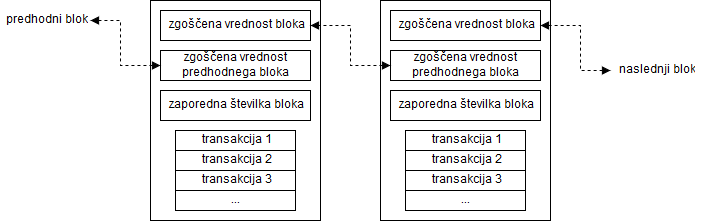
\includegraphics[width=1.0\textwidth]{slike/blockchain.png}
	\caption{Podatkovna veriga}
	\label{blockchain}
\end{figure}

Kombinacija teh pristopov omogoča, da nobena izmed sodelujočih entitet ne more spreminjati že zapisanih blokov.
Napad na omrežje je možen le s prevzemom več kot polovice vseh sodelujočih entitet v omrežju, ki bi potrjevale resničnost ponarejenih transakcij in sčasoma sestavile daljšo podatkovno verigo, ki bi obveljala kot trenutna resnica.
Takšnemu okolju lahko zaupamo, brez centralne avtoritete, ki bi ji zaupali vsi sodelujoči.

Za interakcijo z glavno knjigo in zapisovanje novih informacij omrežje uporablja t. i. pametne pogodbe.
To je del programske kode, ki se lahko odziva na dogodke v omrežju, izvede zapisano poslovno logiko, ter ustvarja nove transakcije \cite{hyperledgerDocs}.

V nadaljevanju tega poglavja se bomo posvetili osnovnim konceptom ter predstavili posebnosti dveh implementacij te tehnologije -- omrežji Ethereum in Hyperledger Fabric.
Osredotočili smo se predvsem na ti dve, ker do rešitve problema pristopata z nasprotnih bregov.
Prva rešitev predpostavlja popolnoma javno omrežje, kjer so identitete uporabnikov neznane, druga svoje prednosti gradi na predpostavki popolnega zaupanja med sodelujočimi identitetami.
V želji zgraditi sistem, ki bo omogočal decentralizirano izvajanje storitev in preprečeval morebitne poneverbe izvedbe posameznih operacij, hkrati pa zagotavljal popolnoma anonimnost udeležencev, je verjetno smiselno uporabiti nekakšno fuzijo obeh pristopov.

\section{Razlaga osnovnih konceptov}

\subsection{Porazdeljena glavna knjiga}
V osrčju tehnologije podatkovnih blokov je porazdeljena glavna knjiga, ki hrani zapise o vseh transakcijah, izvedenih na omrežju.
Glavna knjiga je replicirana na vseh entitetah v omrežju, ki med sabo sodelujejo in skrbijo za vzdrževanje.
Informacije se v glavno knjigo dodajajo z uporabo kriptografskih tehnik, ki zagotavljajo, da je vsaka zapisana transakcija trajna in nespremenljiva.
V glavno knjigo lahko podatke le dodajamo, brisanje in popravljanje obstoječih transakcij ni možno.
To omogoča enostavno preverjanje izvora informacije, od tu tudi drugo poimenovanje za tehnologijo podatkovnih blokov kot sistem dokazovanja (ang. system of proof) \cite{hyperledgerDocs}.
Vsak morebitni napadalec bi moral spremeniti vse naslednike bloka, ki ga želi spremeniti, ter to početi hitreje kot vsi preostali udeleženci skupaj \cite{hampton2016understanding}.

\subsection{Pametne pogodbe}
Pametne pogodbe omogočajo nadzorovan dostop in interakcijo z glavno knjigo.
So osnovni mehanizem za enkapsulacijo informacij in njihovo preprosto vzdrže\-vanje preko omrežja.
Poleg tega omogočajo tudi določeno stopnjo samodejnosti, kot je izvrševanje transakcij brez človeškega posredovanja.
V primerjavi s tradicionalnimi pogodbami nam pametne pogodbe zagotavljajo višjo stopnjo varnosti in zmanjšujejo dodatne stroške, ki so povezani z njihovim izvajanjem \cite{atzei2017survey}.
Leta 1996 je Nick Szabo prvič uporabil izraz pametna pogodba:
\textit{Sam imenujem novodobne pogodbe pametne pogodbe, ker so uporabnejše kot njihove papirne različice.
Pametna pogodba namreč vsebuje digitalno določena zagotovila in protokole, ki jim sledijo vse pogodbene stranke \cite{szabo1996smart, balanticd}.}

Na sliki \ref{smart_contract} je prikazan osnovni potek interakcije pametne pogodbe z glavno knjigo.

\begin{figure}[h]
	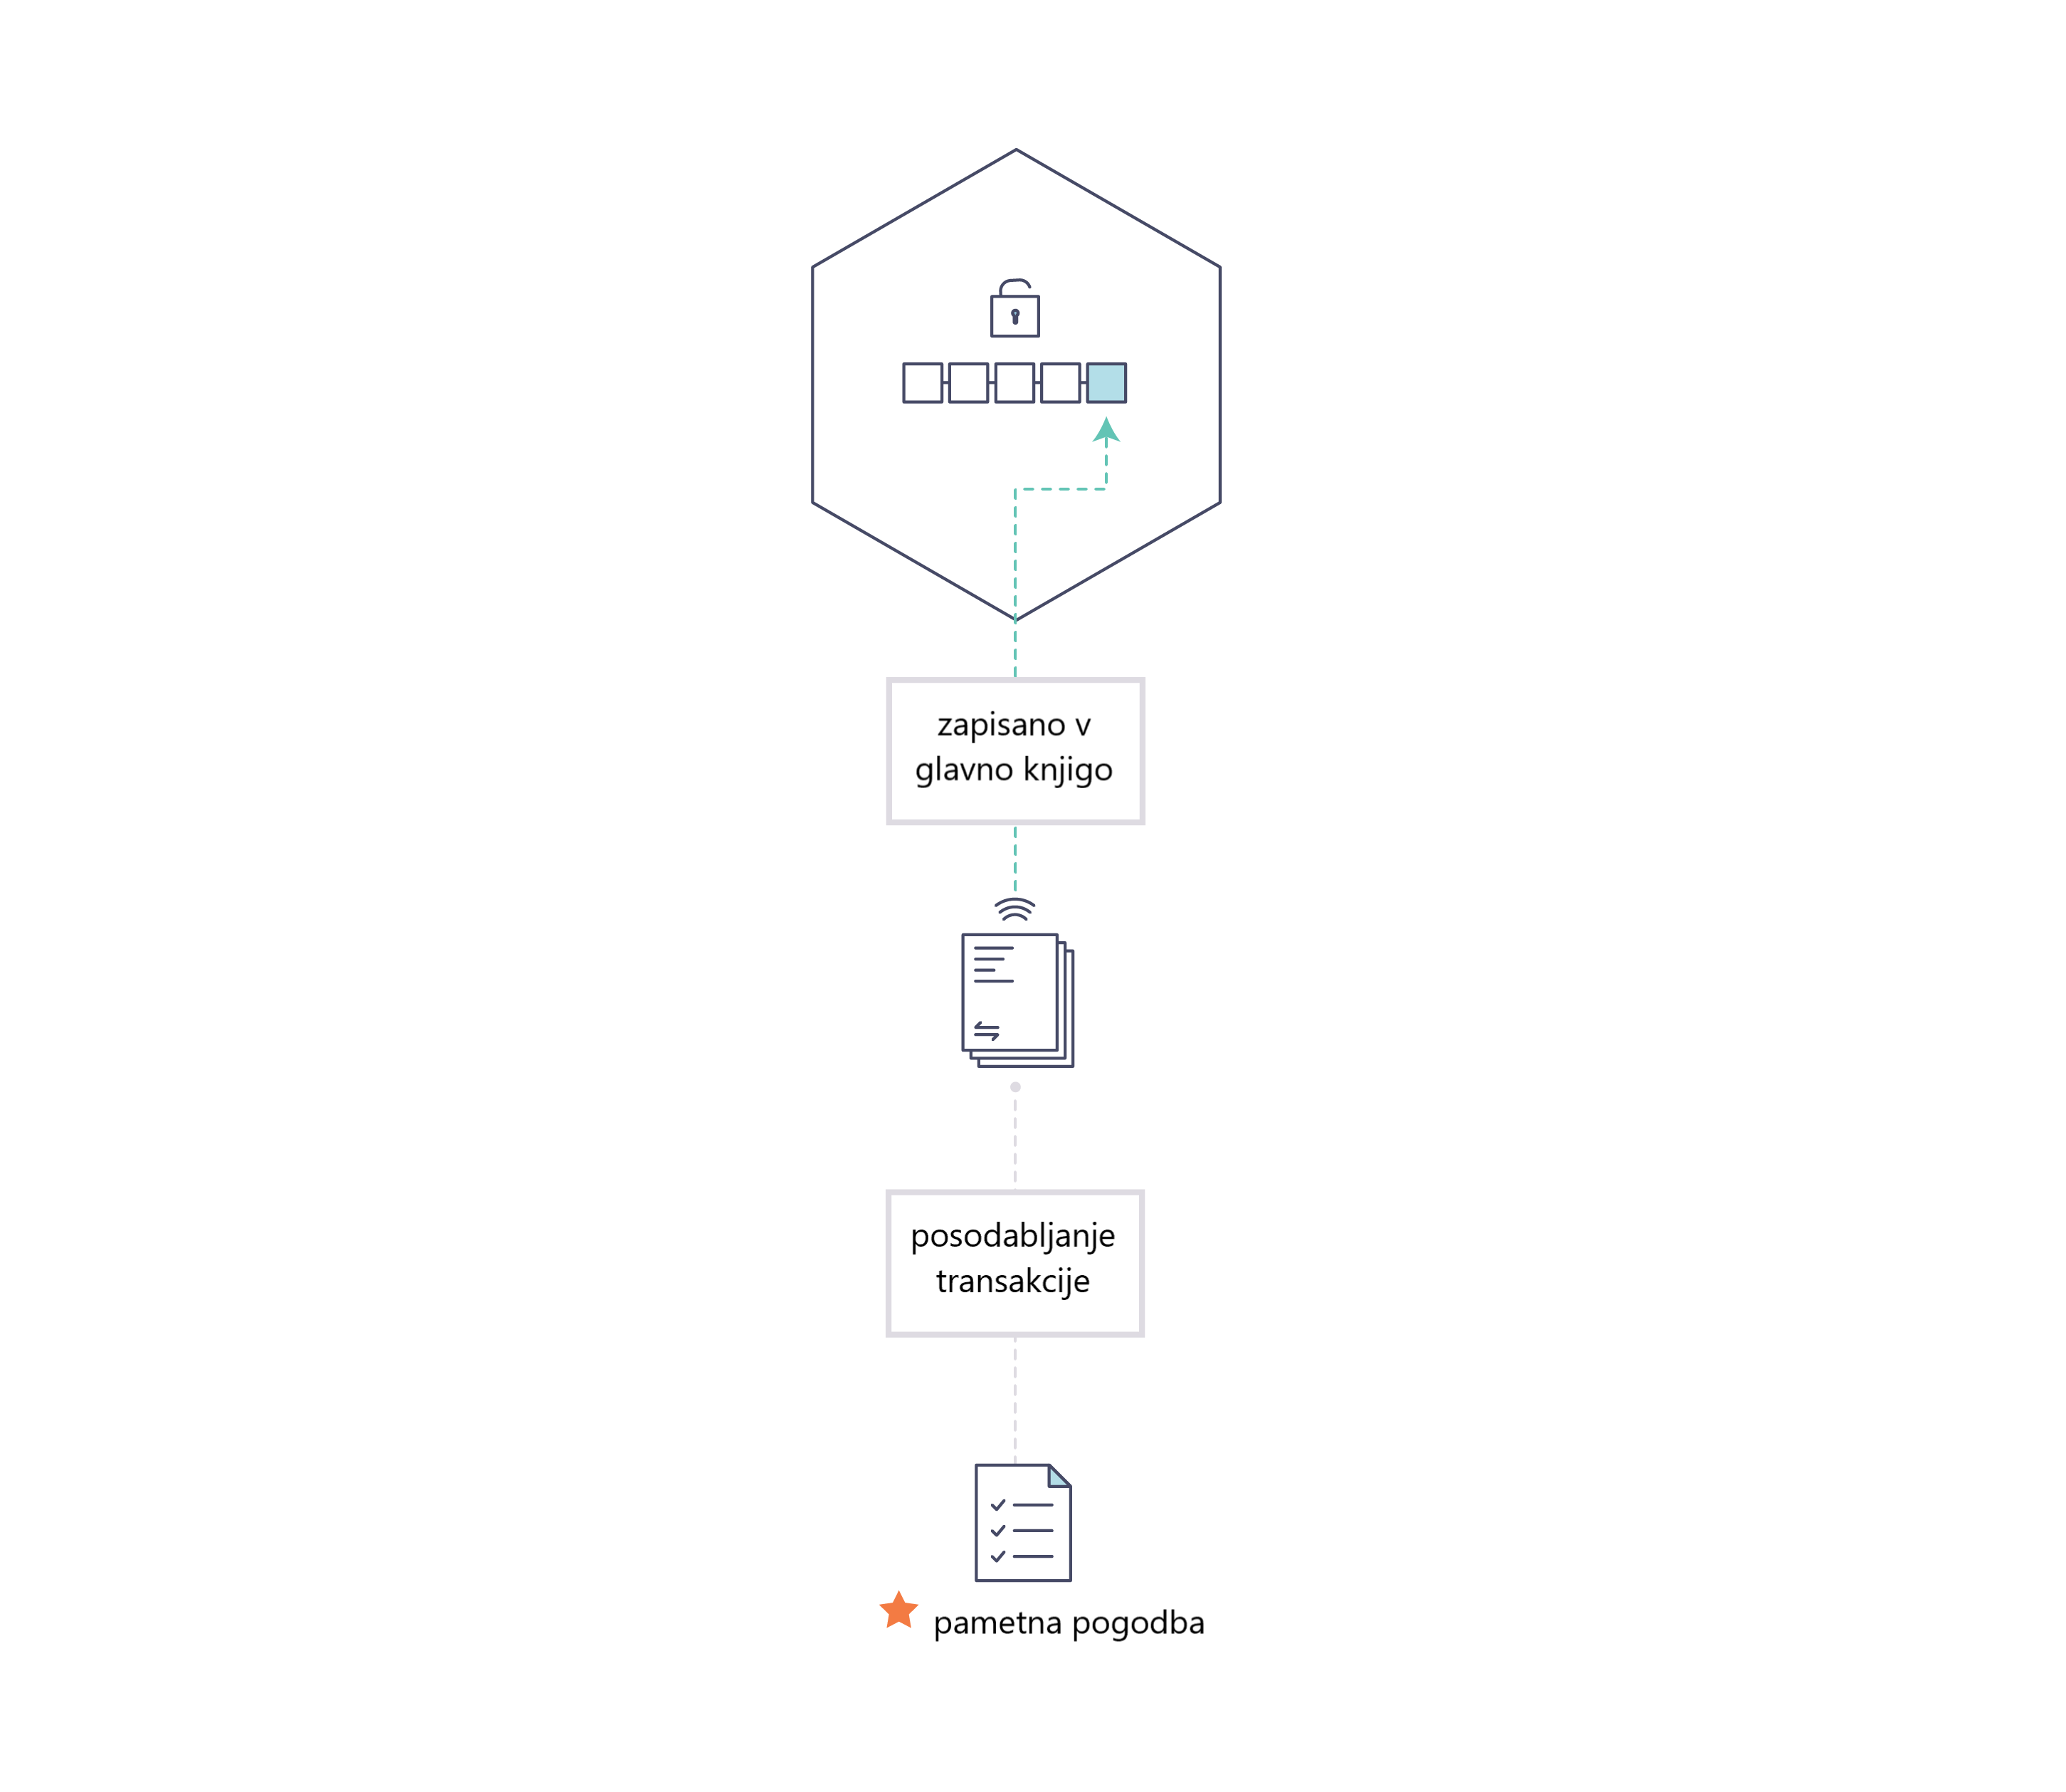
\includegraphics[width=1.0\textwidth]{slike/Smart_Contract_sl.png}
	\caption{Interakcija pametne pogodbe z glavno knjigo \cite{hyperledgerDocs}.}
	\label{smart_contract}
\end{figure}


\subsection{Soglasje}
Proces sinhronizacije glavne knjige v omrežju je imenovan soglasje (ang. consensus).
Zagotavlja, da se glavna knjiga posodobi le takrat, ko so transakcije in podatkovni bloki potrjeni s strani zaupanja vrednih udeležencev omrežja.
Glavna knjiga se posodobi tako, da vsi udeleženci omrežja izvedejo enake (zapisane) transakcije v istem vrstnem redu.
Slika \ref{consensus} prikazuje primer doseženega soglasja.

\begin{figure}[h]
	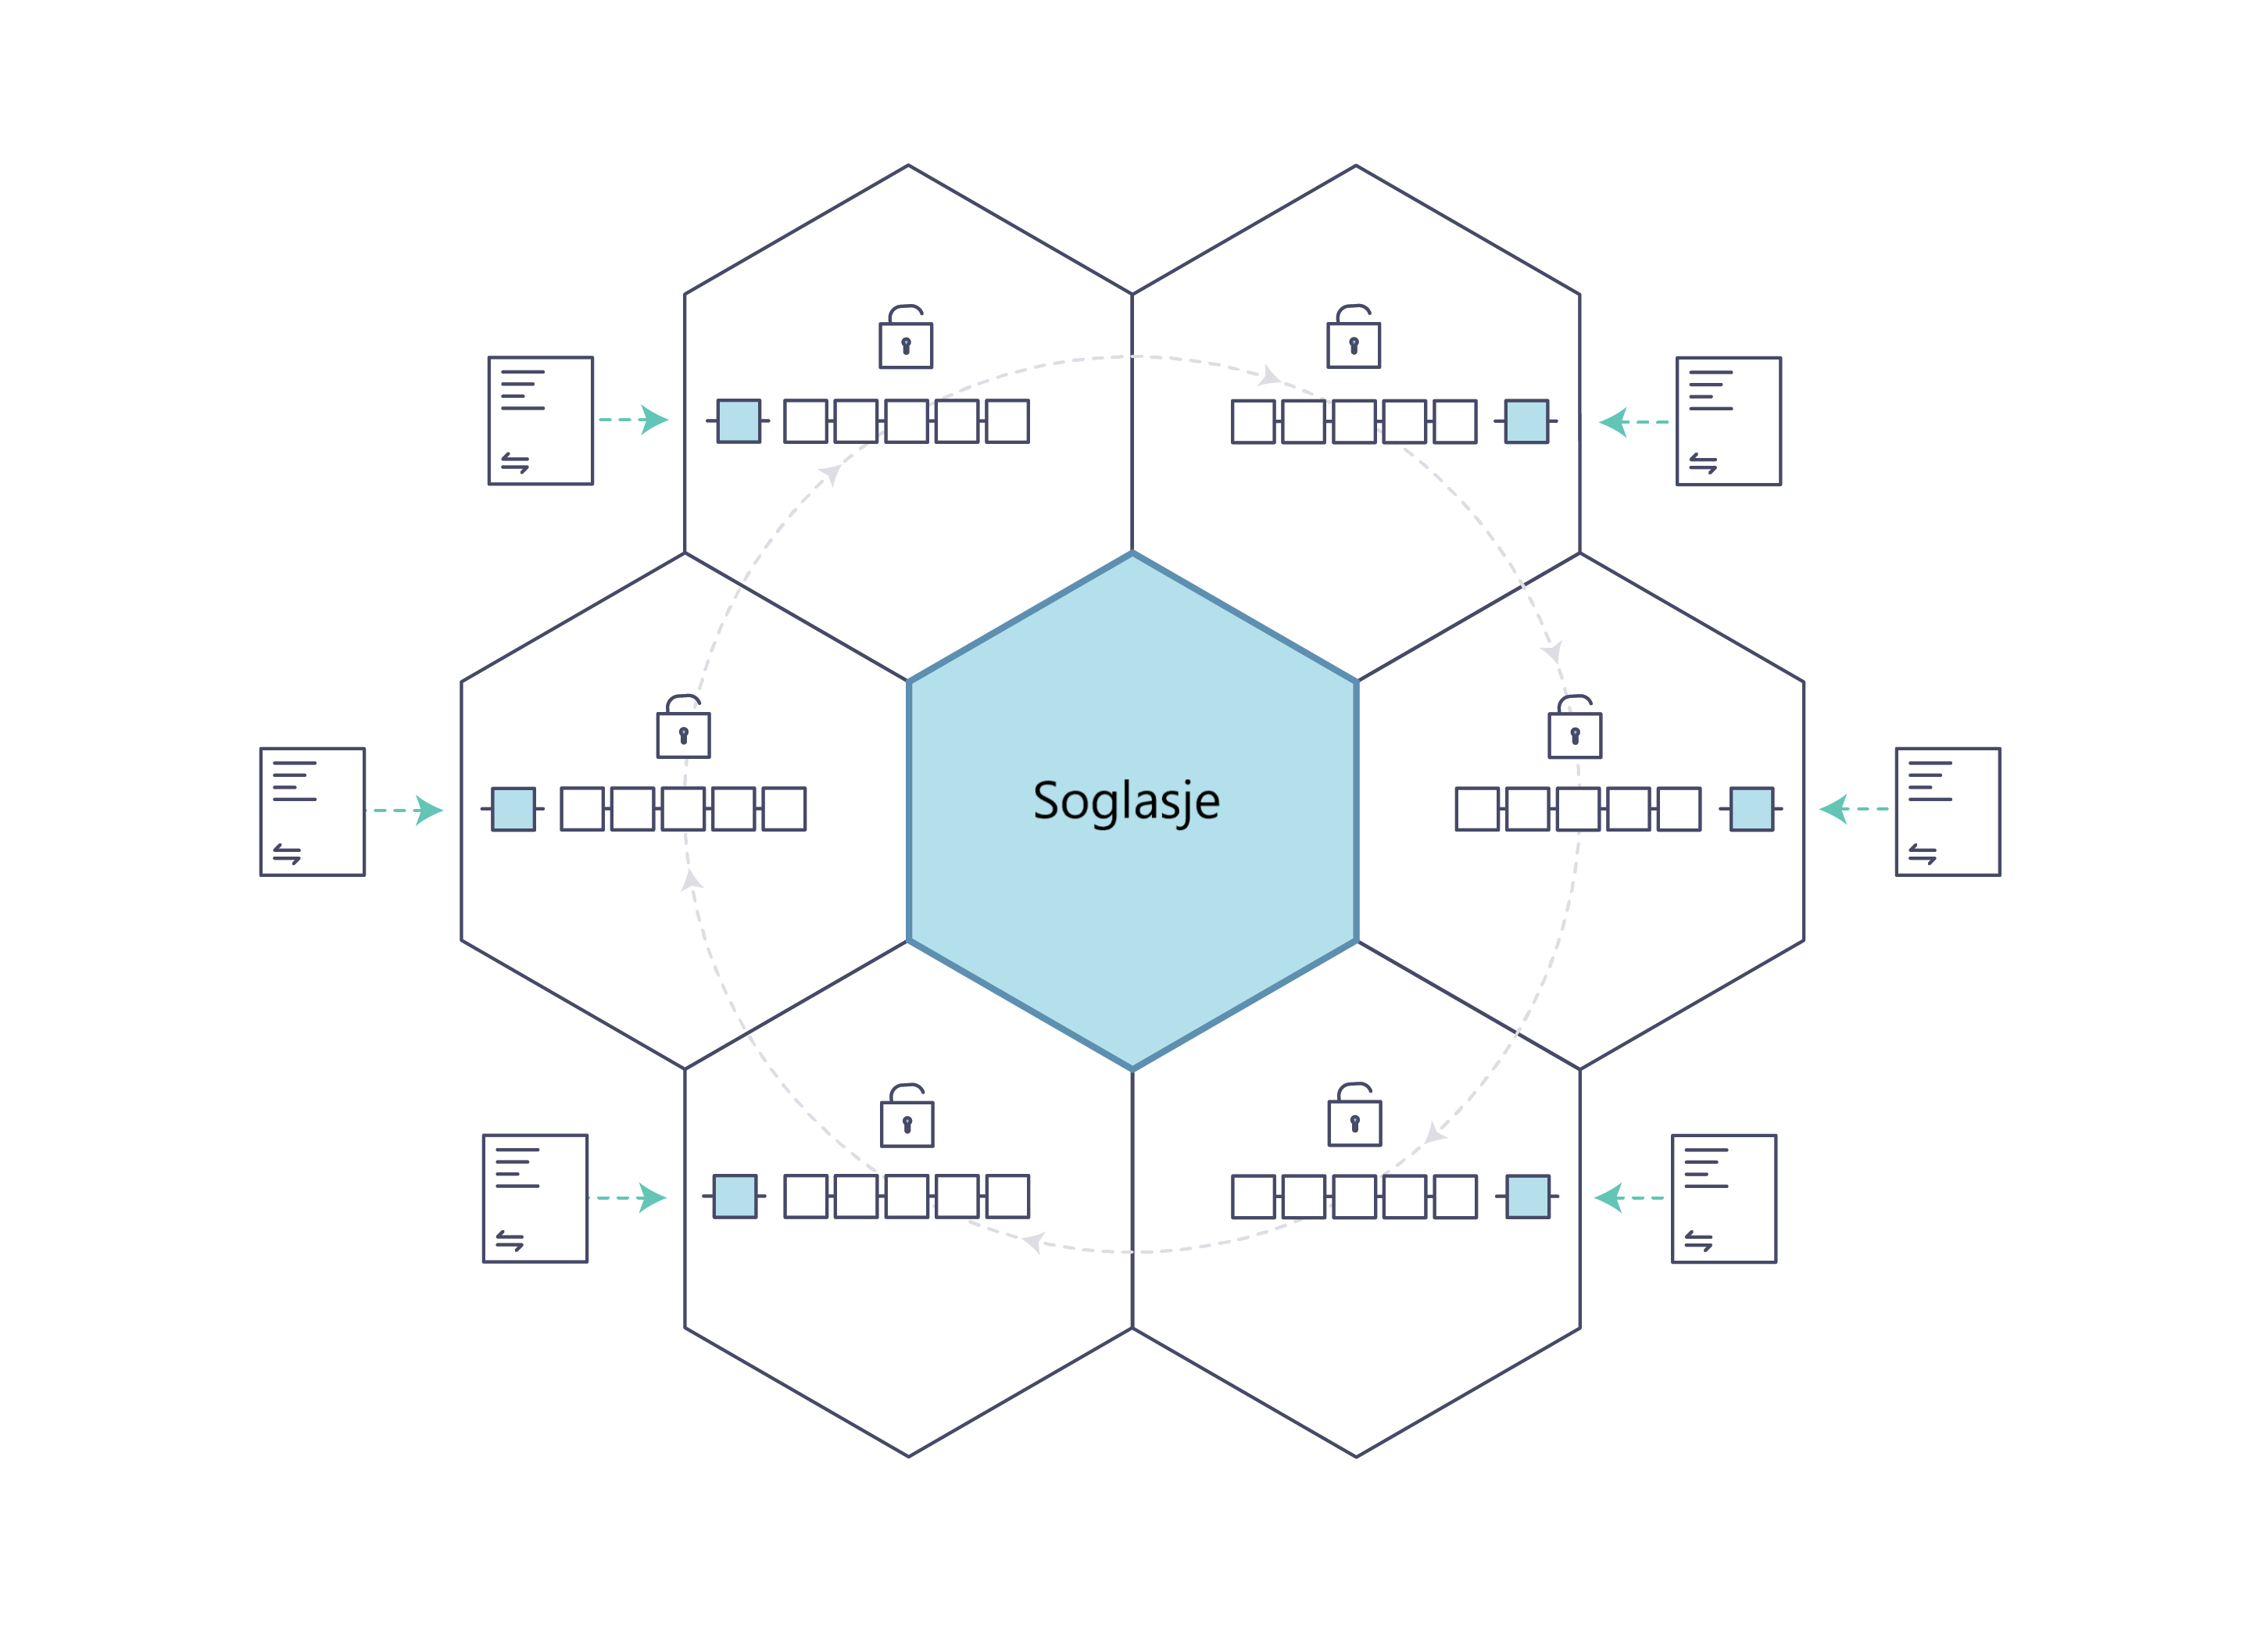
\includegraphics[width=1.0\textwidth]{slike/consensus.png}
	\caption{Doseženo soglasje v omrežju \cite{hyperledgerDocs}.}
	\label{consensus}
\end{figure}


\subsection{Izvajalna okolja glede na zaupanje med udeleženci}
V grobem lahko, glede na stopnjo zaupanja, ločimo dva tipa izvajalnih okolij, ki ga udeleženci delijo med seboj.
Imamo omrežje, kjer so udeleženci vnaprej znani, identificirani s strani tretje osebe, ki ji zaupajo vsi sodelujoči.
Interakcije med njimi so varne v smislu prevzemanja odgovornosti.
Morebitna škodoželjnost udeleženca je enostavno kaznovana zaradi fizično overjenih oseb (pravnih ali fizičnih).

V javnih okoljih teh ugodnosti ne uživamo.
V omrežju lahko sodeluje kdorkoli in to povsem anonimno,
med udeleženci tako privzeto velja načelo nezaupanja.
Zaupa se le stanju celotne najdaljše podatkovne verige.
Tipično so za potrjevanje blokov in novih transakcij uporabljene kriptovalute, pridobljene s t. i. postopkom rudarjenja.
Kriptovalute (ang. cryptocurrencies) predstavljajo plačilno sredstvo za opravljeno računsko delo entitete, ki potrjuje opravljeno transakcijo.
Ta omrežja večinoma temeljijo na Byzantine Fault-Tolerance (BFT) \cite{hyperledgerDocs, castro1999practical}.
Byzantine Fault-Tolerance je algoritem za dosego soglasja med sodelujočimi entitetami, med katerimi ne velja načelo zaupanja in  predpostavlja nezanesljiv prenosni medij.

\subsection{Zasebnost in zaupnost}
Javne podatkovne verige so replicirane na vseh sodelujočih entitetah, kar prinaša transparentnost, obenem pa poslovnim subjektom onemogoča učinko\-vito sklepanje dodatnih ugodnosti, aneksov ipd. s poslovnimi partnerji.
Ena od možnih rešitev problema bi bila šifriranje podatkov, ki pa v tem primeru ni najbolj primerno in varno.
Vsak izmed sodelujočih ima dostop do celotne glavne knjige, kar omogoča napade s silo nad šifriranimi podatki.
V nadaljevanju predstavljeno omrežje Fabric tu vpeljuje koncept kanalov.
Ti predstavljajo logično grupiranje posameznih entitet in omejujejo dostop do pametnih pogodb in glavne knjige na posameznem kanalu \cite{hyperledgerDocs}.

V nadaljevanju bomo predstavili omrežji Ethereum in Hyperledger Fabric.
Prvo je predstavnik javnega omrežja, podatkovna veriga se v celoti replicira na vse sodelujoče udeležence, katerih identitete niso preverjene.
Hyperledger Fabric zaupnost naslavlja drugače in želi zagotoviti preverljivo identiteto posameznega udeleženca v omrežju, največkrat vezano na fizično identiteto.
Ta razlika v zasnovi za seboj prinese dodatne mehanizme preverjanja v omrežju Ethereum, ki pri omrežju Hyperledger Fabric niso nujno potrebna.

\section{Ethereum}
Ethereum je decentralizirana platforma, ki izvaja pametne pogodbe (ang. smart contracts) -- aplikacije.
Platforma je osnovana na verigi podatkovnih blokov, ki omogoča reprezentacijo in prenos vrednosti.
Ethereum si lahko predstavljamo kot svetovni računalnik, izvajanje programske kode pa poteka na vseh sodelujočih računalnikih.
Pametne pogodbe ponujajo možnost interakcije s podatkovno verigo, določeni deli kode pa se izvajajo le pod vnaprej programiranimi pogoji \cite{ethereumWhitepaper}.
Vsaka interakcija s podatkovno verigo je preverljiva in ponovljiva, omrežje pa zahteva večinsko potrjevanje spremembe, ki jo želimo zapisati v verigo.
Potrjevanje transakcij je podrobneje predstavljeno v podpoglavju \ref{confirmTxSub}.

Stanje v omrežju Ethereum določajo objekti, znani kot uporabniški računi (ang. accounts).
Vsak račun sestavlja 20 bajtov dolg naslov, prenos sredstev in informacij med računi pa predstavlja spremembo trenutnega stanja.
Uporabniške račune sestavljajo štiri polja \cite{ethereumWhitepaper}:
\begin{itemize}
\item \textbf{števec (ang. nonce)}, ki preprečuje podvajanje transakcij
\item \textbf{trenutno stanje Ethra (ang. ether balance)} trenutna količina ethra v lasti računa
\item \textbf{pogodbena koda (ang. contract code)} opcijsko polje
\item \textbf{shramba (ang. storage)} privzeto prazno
\end{itemize}

Ether je interno plačilno sredstvo v omrežju.
Uporablja se kot nadomestilo za izvrševanje transakcij.
Ethereum pozna dva tipa uporabniških entitet: zunanje (ang. externally owned), določene s privatnimi ključi, in pogodbene (ang. contract accounts), določene s kodo.
Zunanji računi ne obvladujejo kode, z ostalimi entitetami v omrežju pa lahko komunicirajo preko digitalno podpisanih transakcij.
Pametne pogodbe so entitete, ki se v omrežju odzivajo na vnaprej določena sporočila: izvedejo del logike, berejo in pišejo v glavno knjigo, oziroma pošljejo novo sporočilo v omrežje \cite{ethereumWhitepaper}.

\subsection{Komunikacija med entitetami}
V omrežju obstajata dva načina komunikacije: transakcije (ang. transactions) in sporočila (ang. messages).
Transakcije so podpisani podatkovni bloki, ki jih ustvarijo zunanji uporabniški računi.
Sestavni deli transakcije so:
\begin{itemize}
	\item prejemnik
	\item podpis pošiljatelja
	\item količina prenesenega ethra
	\item podatki (opcijsko)
	\item največje dovoljeno število izvedenih računskih operacij (ang. STARTGAS)
	\item cena posamezne računske operacije (ang. GASPRICE)
\end{itemize}

Sporočila so namenjena interni komunikaciji med pametnimi pogodbami.
So le navidezni objekti, ki obstajajo izključno v izvajalnem okolju.
Sestavlja jih \cite{ethereumWhitepaper}:
\begin{itemize}
	\item pošiljatelj
	\item prejemnik
	\item količina prenesenega ethra
	\item največje dovoljeno število izvedenih računskih operacij (ang. STARTGAS)
\end{itemize}

\subsection{Solidity}
Solidity je jezik, v katerem ustvarjalci omrežja Ethereum priporočajo implementacije pametnih pogodb.
Je visoko nivojski jezik, precej podoben JavaScriptu in namenjen izvajanju na navideznem stroju Ethereum (EVM).
Med konstrukti jezika najdemo dedovanje, knjižnice, uporabniško določene tipe in ostale visokonivojske konstrukte.
Namensko orodje za razvoj pametnih pogodb je trenutno le eno, poznano pod imenom Remix IDE, dostopno pa je tudi v spletni različici \cite{solidityDocs}.

\subsection{Navidezni stroj Ethereum}

Navidezni stroj je glavna abstrakcija celotnega omrežja.
Je izvajalno okolje za pametne pogodbe v omrežju Ethereum in služi kot \sn{peskovnik} za izvajanje kode.
Celotni navidezni stroj lahko predstavimo z n-terko \textbf{(stanje blokov, transakcija, sporočilo, koda, spomin, sklad, programski števec, cena posamezne računske operacije )}.
\textit{Stanje blokov} je predstavitev vseh računov s trenutnim stanjem ethra in shrambe.
Vsaka izvedena operacija zmanjša vrednost preostale količine plina, glede na uteženost posamezne operacije.
Transakcija se zaključi ob izvedbi zadnje operacije v programu oziroma s prekinitvijo, ko porabljena število korakov preseže največjo dovoljeno \cite{ethereumWhitepaper}.


\subsubsection{Potrjevanje in ustvarjanje blokov}
\label{confirmTxSub}
Vsak blok v Ethereum verigi vsebuje kopijo vseh transakcij in zadnjega stanja omrežja.
Poleg tega sta v bloku zapisani tudi zaporedna številka bloka in zahtevnost.
Postopek validacije bloka poteka sledeče:
\begin{enumerate}
\item Preveri, če predhodni blok obstaja in je veljaven.
\item Preveri časovni žig bloka -- biti mora večji od prejšnjega bloka, vendar ne več kot 15 minut v prihodnosti.
\item Preveri številko bloka, zahtevnost, izvor transakcije, izvor \sn{strica} in omejitev količine plina.
\item Preveri veljavnost opravljenega dela (ang. Proof of Work).
\item Naj bo S[0] stanje na koncu predhodnega bloka.
\item Naj bo TX seznam transakcij v bloku in n število transakcij v bloku. Za vsak 
$\{i \mid 0,1,\dots, n-1\}$
je naslednje stanje
 $S[i+1] = APPLY(S[i], TX[i])$.
V primeru napake ali presežene omejitve količine plina na blok (ang. GASLIMIT), vrni napako.
\item Naj $S_{FINAL} = S[n]$. Nagrada za najden blok se izplača samo najditelju.
\item Preveri, da je vrhnje vozlišče Merklovega drevesa stanja $S_{FINAL}$ enaka končnemu stanju v bloku. V tem primeru je blok veljaven.
\end{enumerate}

Koda je izvedena s strani vseh sodelujočih entitet v omrežju \cite{ethereumWhitepaper}.

\section{Hyperledger}
Hyperledger je družina odprtokodnih projektov, namenjenih razvoju tehnologije veriženja podatkovnih blokov.
Projekt deluje pod okriljem organizacije The Linux Foundation v sodelovanju s skupnostjo.
Med prvimi in najbolj znanimi izmed Hyperledger projektov je Hyperledger Fabric, prvotno razvit v podjetjih IBM in Digital Asset.
Pod okrilje projekta Hyperledger spadajo še Sawtooth, Iroha, Burrow ter Indy.
Vsak izmed projektov na svoj način rešuje izzive s področja podatkovnih verig oziroma naslavlja ozko problemsko domeno. Kot primer: projekt Indy se ukvarja s problematiko spletne identitete uporabnika \cite{hyperledgerWeb}.
Trenutno najbolj znana in razširjena platforma je Fabric, v času pisanja dostopna v različici 1.1.
Od ostalih podobnih projektov se loči predvsem s konceptom privatnih omrežji, pri katerih je sodelovanje omejeno s sistemom dovoljenj.
Omogoča modularno izbiro načina soglasja in ga je moč prilagajati zahtevam poslovnih uporabnikov \cite{hyperledgerIbm}.

\subsection{Fabric}
Hyperledger Fabric je v sami zasnovi namenjen poslovni uporabi.
Omogoča modularno in prilagodljivo arhitekturo, podobno kot ostale implementacije tehnologije veriženja blokov pozna tudi pametne pogodbe, tu imenovane \sn{chaincode}.
Pametne pogodbe se izvajajo znotraj vsebnikov Docker in omogočajo implementacijo v poljubnem splošnonamenskem programskem jeziku.
Drugačen je tudi postopek izvedbe transakcije.

Celotno omrežje je zasnovano na predpostavki (delnega) zaupanja med sodelujočimi entitetami, kar ga razlikuje od javnih omrežij.
Enostavna je menjava implementacije protokola za doseganje soglasja, implementiranih bodisi na osnovi reševanja napak ob odpovedi (ang. Crash Fault Tolerant -- CFT) ali bizantinske odpornosti na napake (ang. Byzantine Fault Tolerance -- BFT).
Za samo delovanje ne potrebuje kriptovalute, potrjevanje transakcij in blokov pa ni nujno izvedeno s strani vseh sodelujočih ampak le določene podmnožice.
V teoriji nam omogoča paralelizacijo in posledično višjo zmogljivost celotnega omrežja \cite{hyperledgerDocs}.

\subsubsection{Modularnost}
Omrežje sestavlja šest osnovnih komponent, ki jih je moč poljubno menjati \cite{hyperledgerDocs}:
\begin{enumerate}
	\item Urejevalnik (ang. ordering service).
	\item Upravitelj članstva (ang. membership service) -- povezuje zunanje entitete z njihovimi kriptografskimi predstavitvami.
	\item P2P gossip protocol - opcijski.
	\item Pametne pogodbe (\textit{chaincode}) - procesno izolacijo zagotavlja izvajanje znotraj vsebnikov Docker. 
	Onemogočen je neposreden dostop do glavne knjige.
	\item Sistem za upravljanje podatkovne baze (ang. DBMS).
	\item Zamenljiva politika potrjevanja in validiranja.
\end{enumerate}

\subsubsection{Pametne pogodbe}
Pametne pogodbe so delčki programske kode, ki se izvajajo kot distribuirane aplikacije.
Tri glavne značilnosti teh aplikacij so: veliko število sočasno izvajanih pametnih pogodb, dinamično dodajanje v omrežje in v osnovi nevrednost zaupanja.
Obstoječi načini izvajanja pogodb so umeščeni v arhitekturo uredi-izvedi.
Za njih je značilno, da transakcije validirajo in sekvenčno uredijo, temu pa sledi propagacija potrjenih blokov po omrežju.
Vsaka sodelujoča entiteta nato transakcije izvede v tem vrstnem redu.
Za enoličen način sekvenčnega izvajanja tu nastane potreba po novem, determinističnem programskem jeziku.
En izmed predstavnikov je programski jezik za programiranje pogodb v omrežju Ethereum, Solidity.
Ker je vsaka izmed transakcij izvedena s strani vsake entitete, to predstavlja veliko porabo razpoložljivih virov ter omejuje skaliranje ter učinkovitost izvajanja \cite{hyperledgerDocs}.

Fabric pametne pogodbe izvaja po arhitekturi izvedi-uredi-validiraj.
Vsaka transakcija je najprej izvedena, s čimer se preveri njeno pravilnost.
Nato je urejena glede na protokol za doseganje soglasja.
Ob koncu je transakcija validirana s strani za to pooblaščenih zunanjih entitet.
Tu v igro vstopi domensko specifična politika potrjevanja.
Slednje prinaša potencialno velike performančne prihranke \cite{hyperledgerDocs}.

\section{Tehnologija veriženja podatkovnih blokov v kontekstu decentraliziranega izvajanja}
Decentralizirana hramba podatkov je osnova, na kateri je primerno graditi in osnovati sisteme sposobne decentraliziranega izvajanja.
Raziskave in tehnike uporabe kriptografskih in drugih protokolov, ki zagotavljajo nespremenljivost podatkov in v praksi preprečujejo njihovo ponarejanje, lahko apliciramo nivo višje, na nivo poslovne logike.
Pametne pogodbe lahko primerjamo s shranjenimi procedurami in prožilci v sistemu za upravljanje podatkovne baze.
Poslovna logika je kompleksnejša in decentralizirane storitve se izvajajo na podoben princip kot trenutne storitve, le okolje v katerem se izvajajo je decentralizirano.
Za decentralizirano izvajanje moramo decentralizirati vsako izmed komponent, ki sestavljajo trenutne centralizirane sisteme.
Poleg tega moramo zagotoviti tudi preverljivost samega izvajanja, podobno kot pri pametnih pogodbah.
Trenutno znamo varno hraniti podatke na tisoče napravah ter hkrati zagotavljati njihovo pristnost.
Zamisel o decentraliziranem registru smo osnovali prav na tej lastnosti, kar je podrobneje razloženo v poglavju \ref{ch4}.

\chapter{Decentralizirano izvajanje mikrostoritev}
\label{ch4}

Izvajanje storitev v oblaku s sabo prinaša kar nekaj prednosti, kot so samodejno skaliranje posamezne storitve glede na trenutne zahteve in potrebe.
Računalniški oblak je abstrakcija, ki za seboj skriva ogromne podatkovne in računske centre.
Ti so v večini v lasti velikih korporacij, prednjačijo Amazon, Google in Microsoft.
Odvisnost od ponudnika računalniškega oblaka zna biti problematična.
Pri menjavi ponudnika nastopijo težave pri prenosu storitev med okolji, dostopnost storitev je delno odvisna tudi od tretje osebe. 
Napaka v sistemu lahko povzroči večurno nedostopnost naših storitev.
Navkljub skrbi, ki jo ponudniki posvečajo vzdrževanju stalne dosegljivosti, od zadnjega odmevnejšega primera mineva le dobro leto in pol \cite{awsFail}.

Cilj diplomske naloge je decentralizirati izvajanje storitev.
Vsaka sodelujoča entiteta v omrežju lahko, pod določenimi pogoji, izvaja katerokoli izmed nabora razpoložljivih storitev.
Storitve bomo v nadaljevanju naslavljali z dApi (kot okrajšava za decentraliziran API).
Prednost, ki jo prinaša decentralizirano izvajanje poslovne logike, je praktično nemogoč napad zavrnitve storitve (DOS) in porazdeljen napad zavrnitve storitve (DDOS).
V omenjenih napadih je napadalec zmožen posamezno sodelujočo entiteto v omrežju obremeniti do te mere, da le ta preneha z izvajanjem določene storitve.
Decentraliziran sistem bi v primeru prenehanja izvajanja storitve na eni entiteti izvajanje dodelil drugi.
Postopek bi moral biti za končnega uporabnika omrežja transparenten.
S tehnologijo podatkovnih blokov bi bilo moč posamezne klice storitev tudi finančno ovrednotiti.
Trenutno je potrebnih več klicev, ki najprej izvedejo samo poslovno logiko aplikacije, temu pa sledi klic, ki izvede še finančno transakcijo.
Podatkovna veriga nam omogoča, da klice storitev opremimo s finančnimi podatki in ob uspešni izvedbi izvajalca sistem samodejno nagradi.

V nadaljevanju diplomskega dela so predstavljeni osnovni koncepti rešitve registracije in odkrivanja storitev v decentraliziranem okolju.
Odkrivanje storitev v decentraliziranem okolju igra pomembno vlogo, podobno kot pri storitvah, ki se izvajajo v oblačnih sistemih.
Poleg te komponente za polno delujoč sistem potrebujemo še dodatne mehanizme, ki bodo preverjali pravilnost izvajanja, zbirali metrike in porazdeljevali delo.
Predstavljena rešitev tako prispeva le del funkcionalnosti končnega sistema, ki bo omogočal decentralizirano izvajanje.

\section{Problem zaupanja nevrednega omrežja}
Izvajanje storitev na poljubni napravi v omrežju prinaša problem zagotavljanja pravilnosti izvajanja.
V zasebnih omrežjih so sodelujoče entitete vnaprej znane in njihove digitalne identitete overjene s strani tretje osebe, ki uživa zaupanje vseh sodelujočih strank.
Kot primer, za pridobitev digitalnega certifikata za fizično osebo, se mora le-ta zglasiti na za to pooblaščeni enoti, ki opravi postopek overjanja.
Na ta način pridobimo vez med digitalno in fizično identiteto, vsaka morebitna zloraba v digitalnem okolju prinaša kazensko odgovornost v realnem svetu.
V želji po popolni decentralizaciji želimo odpraviti potrebo po posredniku.
Na podatkovnem nivoju tu v igro vstopajo algoritmi za dosego soglasja, edino resnico na omrežju pa predstavlja najdaljša podatkovna veriga.
Pri decentraliziranem izvajanju moramo, poleg verodostojnosti podatkov, zagotoviti tudi verodostojnost in zanesljivost izvajanja zapisane programske logike.
Problem, ki ga na specifičen način rešuje omrežje Hyperledger Sawtooth \cite{sawtooth}, je potrebno posplošiti in pripraviti za uporabo na poljubni strojni in programski opremi.

\section{Odkrivanje storitev v decentraliziranem okolju}

Odkrivanje storitev je v arhitekturi mikrostoritev pomembno zaradi ogromno različnih vrst storitev, ki so večkrat replicirane, življenjska doba posamezne replike pa je precej kratka.
Statično kodiranje naslovov odvisnih storitev je neprimerno, zato potrebujemo mehanizem dinamičnega odkrivanja trenutno aktivnih storitev.
V centraliziranih sistemih je problem rešen z uporabo centralnega registra storitev (etcd, Consul, ZooKeeper).

Predlagan sistem za odkrivanje storitev v decentraliziranem okolju sestavljajo naslednji mehanizmi:
\begin{itemize}
	\item Registracija aplikacije
	\item Registracija izvajalcev
	\item Registracija dApija
	\item Odkrivanje storitev
\end{itemize}

Registracija in odkrivanje storitve je uporaba že znanih konceptov, prenesenih v okolje, kjer vlogo registra storitev prevzema porazdeljena glavna knjiga.
Dodatno smo uvedli še registracijo aplikacije, ki je pripravljena na izvajanje v decentraliziranem omrežju in registracijo izvajalcev.
Slednja omogoča lastništvo več izvajalnih naprav eni posamezni identiteti.


\subsection{Registracija aplikacije}
\label{registerService}

Omrežje za izvajanje decentraliziranih storitev je javno, kdorkoli lahko objavi in ponudi novo aplikacijo.
Izvorno kodo oziroma izvršljivo datoteko aplikacije shranimo v decentralizirano shrambo.
Temu sledi zapis podatkov (ime, verzija, izvajalno okolje...) o aplikaciji v glavno knjigo.
Ob uspešni registraciji omrežje proži dogodek s podatki o novi aplikaciji.
Izvajalci, ki se registrirajo na te dogodke, lahko takoj pričnejo z izvajanjem, če se za to odločijo, oziroma jim je izvajanje dodeljeno s strani omrežja.
Razporejanje opravil in izvajanja po omrežju sta stvar prihodnjih raziskav.
Preprost diagram poteka je prikazan na sliki \ref{register_api}.

\begin{figure}[h]
	\centering
	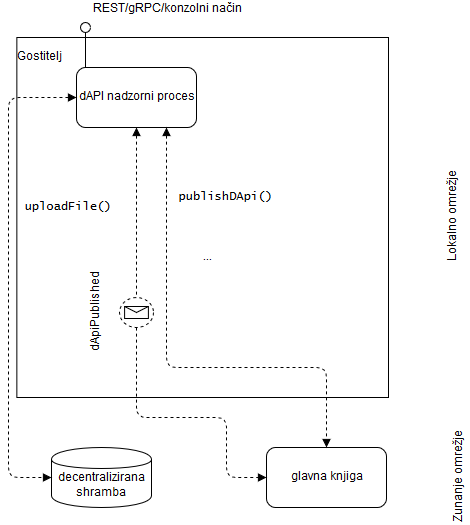
\includegraphics[width=0.8\textwidth]{slike/register_api.png}
	\caption{Registracija nove aplikacije.}
	\label{register_api}
\end{figure}

\subsection{Registracija izvajalcev}
\label{registerWorker}
Vsaka identiteta lahko upravlja z več izvajalnimi enotami.
Ta pristop omogoča enemu uporabniškemu računu pripis vseh nagrad, ki si jih prisluži množica izvajalcev.
Podatki, ki se o posameznem izvajalcu zabeležijo, so: lastnik (ang. account), unikatna številka izvajalca (id) in naslov, preko katerega je izvajalec dosegljiv.
Izvajalcu se lokalno nastavi omejitve glede porabe sistemskih virov, ki jih lastnik nameni decentraliziranemu izvajanju storitev.
Postopek je shematsko prikazan na sliki \ref{register_worker}.

\begin{figure}[h]
	\centering
	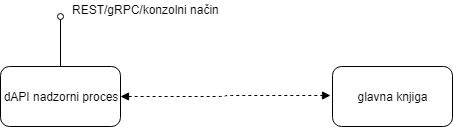
\includegraphics[width=1.0\textwidth]{slike/register_worker.png}
	\caption{Postopek registracije izvajalcev.}
	\label{register_worker}
\end{figure}

\subsection{Registracija izvajanja dApija}
\label{registerExecution}
Ob zahtevi za pričetek izvajanja aplikacije, predhodno registrirane v omrežju, se prične postopek pridobivanja informacij o želenem dApiju.
Iz registra se pridobi podatke o imenu, verziji, lastniku in lokaciji shrambe aplikacije.
Izvorno kodo oz. izvršljivo datoteko dApija se pridobi iz omrežja, po potrebi jo nadzorni proces za izvajanje dApijev prevede in zažene.
Storitev sama ob inicializaciji poskrbi za registracijo v registru (glavna knjiga).
Zabeleži se podatke o izvajalcu in dApiju, ki je pričel z izvajanjem.
Gre za najbolj kompleksen del registracije, shematsko je prikazan na sliki \ref{register_service}.

\begin{figure}[h]
	\centering
	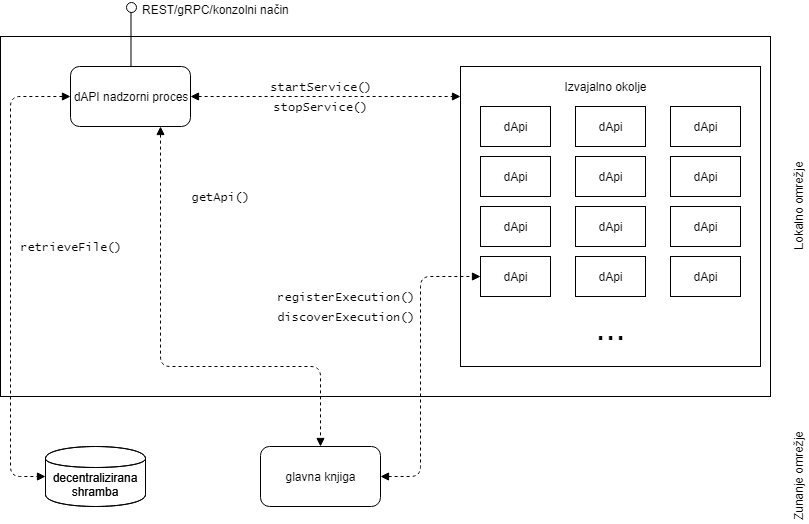
\includegraphics[width=0.8\textwidth]{slike/register_service.png}
	\caption{Postopek registracije izvajanja storitve.}
	\label{register_service}
\end{figure}

\subsection{Odkrivanje dApijev}
\label{serviceDiscovery}
Želen dApi, pod pogojem da se v omrežju izvaja, pridobimo z enostavno poizvedbo v glavni knjigi.
Med razpoložljivimi izvajalci odjemalec izbere enega, pridobi podatke o lokaciji izvajanja in izvede klic (slika  \ref{discover_service}).
Od tu naprej komunikacija med storitvami poteka preko izbranega protokola (REST, gRPC, event driven itd.).

\begin{figure}[h]
	\centering
	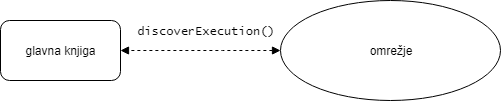
\includegraphics[width=0.8\textwidth]{slike/discover_service.png}
	\caption{Postopek odkrivanja.}
	\label{discover_service}
\end{figure}

Odjava dApija predstavlja težji del naloge, ker ni centralnega procesa, ki bi bdel nad registriranimi dApiji in preverjal njihovo dosegljivost.
V centraliziranem sistemu register storitev skrbi za seznam aktivnih storitev in registrirane storitve spremlja, ter jih ob neodzivnosti odstrani iz seznama.
Glavna knjiga, ki tu predstavlja register storitev, ni samostojen proces, ki bi vzdrževal aktualen seznam aktivnih storitev.
Potrebno bo dodatno raziskovalno delo, kako učinkovito odjaviti storitev, podobno kot je to rešeno pri trenutno uporabljenih registrih (etcd, Consul, ZooKeeper).
Možne rešitve so naključno preverjanje storitev s klicem vnaprej dogovorjene dostopne točke oziroma periodično preverjanje s strani za to določenih entitet.
Za odjavo posamezne storitve je tako zaenkrat odgovoren nadzorni proces.

\chapter{Implementacija predlagane rešitve}
\label{ch5}

V okviru razvoja celostnega ogrodja za decentralizirano izvajanje mikrostoritev smo se osredotočili le na osnovne funkcionalnosti registra storitev -- registracijo aplikacije, registracijo izvajalcev, registracijo ter odkrivanje dApija.
Polno delujoč register sestavljajo še preverjanje odzivnosti storitev in posodabljanje stanja registra, kar v trenutni različici projekta ni podprto.

\begin{figure}[h]
	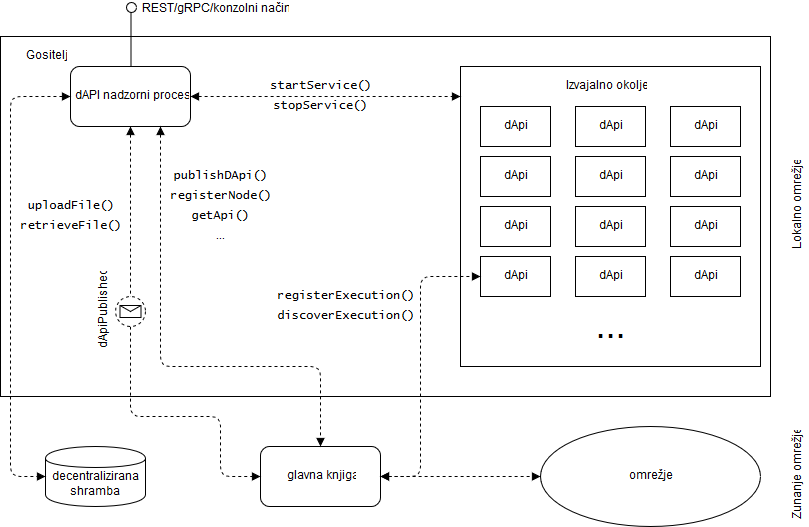
\includegraphics[width=0.8\textwidth]{slike/dApi_sl.png}
	\caption{Arhitekturna shema rešitve.}
	\label{scheme}
\end{figure}

Na sliki \ref{scheme} je prikazana shema predlagane rešitve.
Osrednji del omrežja je nadzorni proces -- \textit{dApi manager}, ki dostopa do glavne knjige, decentralizirane shrambe in upravlja z dApiji, ki jih gostitelj izvaja.
Nadzorni proces v trenutni različici podpira upravljanje z vsebniki Docker.
Aplikacije, ki so na voljo za izvajanje, so shranjene na datotečni shrambi IPFS, podporna podatkovna veriga je na omrežju Ethereum.
Posamezne komponente sistema so podrobneje opisane v nadaljevanju.

\section{Nadzorni proces}
Nadzorni proces za izvajanje decentraliziranih storitev (dApijev) skrbi za:
\begin{itemize}
	\item registracijo novih storitev v omrežje, 
	\item prenos izvršljivih datotek v in iz omrežja,
	\item zagon, zaustavitev in upravljanje storitev.
\end{itemize}

Komunikacija z nadzornim procesom trenutno poteka preko aplikacijskega vmesnika REST, v načrtu pa je implementacija vmesnikov za konzolni nadzor ter podpora novejšim komunikacijskim protokolom kot so gRPC, Apache Trift in podobni.
Nadzorni proces se izvaja na gostiteljski napravi.

Za registracijo nove aplikacije nadzornemu procesu podamo pot do slike vsebnika Docker.
Sistem poskrbi za distribucijo slike v omrežje IPFS in podatke o storitvi doda v shrambo pogodbe na omrežju Ethereum.
Ob uspešni registraciji se sproži dogodek, ki sodelujoče izvajalce obvesti o novi aplikaciji, pripravljeni za izvajanje.
Te se na dogodek lahko odzovejo z zahtevo za pričetek izvajanja dApija.
Trenutno je izvajanje novega dApija potrebno sprožiti ročno, ko bo pripravljen modul za razporejanje opravil, bo postopek v celoti avtomatiziran.
Želeno aplikacijo se pridobi iz omrežja IPFS, sliko vsebnika se naloži v izvajalno okolje Docker in zažene.
dApi sam poskrbi za registracijo in odkrivanje ostalih storitev v omrežju.

Implementacijo nadzornega procesa za dApije smo izvedli z uporabo ogro\-dja KumuluzEE.
KumuluzEE je odprtokodno ogrodje za razvoj mikrostoritev s tehnologijami Java EE.
Ogrodje nam omogoča enostaven prehod iz monolitne arhitekture v arhitekturo mikrostoritev \cite{kumuluzee}.
Izvajanje storitve se izvede preko konfiguracijske datoteke, ki smo jo za potrebe decentraliziranega izvajanja dopolnili (\ref{conf}):

\begin{lstlisting}[caption={Razširitev konfiguracijske datoteke},captionpos=b,label={conf}]
dapi-manager:
  storage:
    remote:
      type: ipfs
      location: /ip4/127.0.0.1/tcp/5001
    local:
      downloadFolder: download
  execution:
  	managers:
  	- type: docker
	    connection: tcp://192.168.99.100:2376
	    tls: true
	    certificate-path: /path/to/certificate
	    instance-limit: 10
  blockchain:
    provider: ethereum
    host: http://127.0.0.1:8545
    account: /path/to/wallet
    password: password
\end{lstlisting}

Konfiguracijo sestavljajo osnovni podatki, potrebni za delovanje nadzornega procesa.
Podana je pot do decentralizirane in lokalne shrambe, naslov izvajalnega okolja za vsebnike ter naslov procesa, ki izvaja protokol Ethereum.

\section{Decentralizirana shramba}
Izvršljive datoteke oziroma slike vsebnikov storitve je potrebno shraniti na način in lokacijo, kjer bodo dostopne vsem sodelujočim entitetam v omrežju.
Podobno, kot želimo izvajanje storitev decentralizirati, želimo poskrbeti tudi za decentralizirano shrambo.
V implementaciji smo uporabili shrambo IPFS.
Gre za projekt, osnovan na omrežju Ethereum, glavni cilj pa je shranjevanje datotek v porazdeljeni shrambi.
Dostop do datotek poteka prek omrežja P2P, protokol za izmenjavo datotek BitSwap je podoben protokolu BitTorrent.
Vsako datoteko, ki jo želimo shraniti v omrežje, odjemalec razbije na podatkovne bloke, izračuna zgoščeno vrednost posameznega bloka, te vrednosti za tem sestavi v strukturo imenovano Merkle Tree.
Datoteko pridobimo enostavno preko zgoščene vrednosti v korenu drevesa.
Omrežje je sposobno poiskati posamezne koščke prvotne datoteke in njeno vsebino hitro preveriti z izračunom zgoščene vrednosti. 
V kolikor nam kdo želi podtakniti napačne bloke posamezne datoteke, sistem to prepozna in neveljavne bloke preprosto zavrže, ko od ostalih sodelujočih entitet prejme iste dele datoteke.
Datoteka je veljavna, v kolikor sistem uspe sestaviti podatkovno strukturo Merkle Tree, pri katerem je korenska zgoščena vrednost identična podani \cite{Ipfs}.

\section{Odjemalec za omrežje Ethereum}
Sistem za delovanje potrebuje odjemalca, ki se zna povezati v omrežje Ethereum.
V naši testni postavitvi je mesto odjemalca prevzel program Geth, implementacija protokola Ethereum v programskem jeziku Go \cite{Geth}.
Nadzorni proces se preko JSON RPC povezuje na lokalno instanco odjemalca Geth, decentralizirane storitve v izvajalnem okolju Docker pa se 
povezujejo na proces, dostopen preko mreže Infura.
Infura nam omogoča enostaven dostop do omrežja Ethereum brez potrebe po lokalnem izvajanju protokola Ethereum.
Za sodelovanje v omrežju nam tako lokalno ni potrebno namestiti ničesar, prav tako nam ni potrebno hraniti
celotne zgodovine podatkovne verige. 
Na spletni strani se enostavno registriramo, s tem pridobimo unikaten ključ, ki nam omogoča dostop do oddaljenega izvajalca \cite{Infura}.

\section{Implementacija pametne pogodbe}
Pametna pogodba, ki predstavlja register storitev in osrednji del sistema, je napisana v programskem jeziku Solidity.

Osnovni konstrukti zasnovane pogodbe so strukture User, dApi, Worker in Execution (\ref{user}).

\begin{lstlisting}[caption={Osnovni konstrukti pametne pogodbe za decentraliziran register storitev},captionpos=b,label={user}]
contract Registry {
	struct User {
		string friendlyName;
		mapping(bytes32 => Worker) workers;
		mapping(bytes32 => dApi) dApis;
	}
	
	struct dApi {
		string name;
		string version;
		string location;
		bool isValid;
	}
	
	struct Worker {
		string name;
		bytes32 workerId;
		bool isValid;
	}
	
	struct Execution {
		Worker worker;
		string location;
		bool active;
	}
	
 	/// MAPPINGS
	mapping (address => User) users;
	mapping (bytes32 => Execution[]) dApiExecutors;
	...
\end{lstlisting}

Struktura \textbf{User} predstavlja ponudnika decentraliziranih aplikacij.
Vsakemu ponudniku pripada seznam izvajalcev (ang. workers) in objavljenih APIjev (dApis).
O posameznem dApiju hranimo ime, verzijo ter lokacijo, ki v našem primeru predstavlja zgoščeno vrednost korena slike Docker, shranjene na IPFS.
Vsak izvajalec je samostojna enota, ki je zadolžena za izvajanje aplikacije, struktura Execution, v navezavi s preslikavo \textit{dApiExecutors}, pa povezuje aplikacijo z njenimi izvajalci in naslovom, preko katerega je dostopna.

Registracija poteka v več korakih, najprej je potrebno registrirati ponudnika storitve, nato se samodejno ob zagonu instance nadzorne storitve izvede registracija izvajalca.
Nadzorna storitev predstavlja enega izvajalca, ta pa skrbi za eno ali več storitev.
Za registracijo storitve poskrbi storitev sama, preko razširitve za ogrodje KumuluzEE \textit{Kumuluz-dapi}, ki je opisana v nadaljevanju (\ref{registerAPI_f}).

\begin{lstlisting}[caption={Funkcija za registracijo APIja},captionpos=b,label={registerAPI_f}]
function registerApi(string _name,
	string _version,
	string _location,
	bytes32 _hash, bool _isValid) public {
	dApi memory dapi = dApi(
	_name,
	_version,
	_location,
	_isValid
	);
	
	users[msg.sender].dApis[_hash] = dapi;
	emit dApiPublished(_name, _version, msg.sender,
	_hash);
}
\end{lstlisting}

Proces odjave izvajanja storitve je kompleksnejši postopek, ki zahteva kar nekaj računskega dela (\ref{deregisterService_f}).
Dokler je v sistemu malo registriranih izvajalnih enot je odjava hitra in za uporabnika neopazna, tako z vidika časa kot cene.
Problem nastopi v primeru velikega števila izvajalnih enot.
Podatki o izvajalni enoti so shranjene v polju.
Na testnem omrežju \textit{Rinkeby} smo ob testiranju večjega števila registriranih izvajalnih enot presegli omejitev računskih korakov na transakcijo (ang. gas).
Vzrok za preseženo dovoljeno računsko zahtevnost je zanka, ki poišče storitev, ki jo želimo odjaviti.

\begin{lstlisting}[caption={Odjava izvajanja},captionpos=b,label={deregisterService_f}]
function deregisterExecution(bytes32 _apiHash, 
uint _wIndex) public {
	if (_wIndex >= dAPIExecutors[_apiHash].length)
		return;
	
	for (uint i = _wIndex;
	i<dApiExecutors[_apiHash].length-1; i++){
		dApiExecutors[_apiHash][i]=
			dApiExecutors[_apiHash][i+1];
	}
	dApiExecutors[_apiHash].length--;
}
\end{lstlisting}

Računsko še zahtevnejši problem nastopi ob odjavi izvajalca, tu bi bilo potrebno iterirati preko vseh registriranih storitev in poiskati izvajalca za brisanje.
Ta del registra še ni implementiran in potrebuje dodatno pozornost v prihodnje.


\section{Razširitev platforme KumuluzEE za podporo decentraliziranim aplikacijam}

\subsection{Implementacija Kumuluz-dapi}
Želja in cilj za učinkovit razvoj decentraliziranih aplikacij je priprava programskih vmesnikov, ki bodo razvijalcem omogočili enostavno nadgradnjo in predelavo obstoječih aplikacij v dApije.
Trenutno razvijamo razširitev za aplikacije, ki uporabljajo platformo KumuluzEE.
Vmesnik mora biti intuitiven in enostaven za uporabo, zato smo za zgled vzeli podobno in že obstoječo rešitev \textit{KumuluzEE Discovery}, ki rešuje problem odkrivanja storitev v oblačnih arhitekturah \cite{maldip}.

\subsubsection{Anotacije}
Razširitev vsebuje anotaciji, s katerima opremimo obstoječo aplikacijo.
Prva služi registraciji storitve, z njo pa se opremi glavni aplikacijski razred storitve REST, ki je trenutno edini podprt način komunikacije (\ref{annotationReg}).

\begin{lstlisting}[caption={Anotacija za registracijo storitve},captionpos=b,label={annotationReg}]
@Qualifier
@Retention(RetentionPolicy.RUNTIME)
@Target({ElementType.TYPE})
public @interface RegisterDApi {
	String name() default "";
	String environment() default "";
	String version() default "";
	ApiType apiType() default ApiType.REST;
}
\end{lstlisting}

Podatki, ki jih beležimo o posamezni storitvi so: \textit{ime (ang. name), okolje (ang. environment), verzija (ang. version) in tip aplikacijskega vmesnika (ang. apiType)}.


Druga anotacija skrbi za označevanje parametrov, ki jih preko javanske tehnologije CDI, vrinemo v spremenljivke (\ref{annotationD}).

\begin{lstlisting}[caption={Anotacija za odkrivanje storitve},captionpos=b,label={annotationD}]
@Qualifier
@Target({ElementType.FIELD, ElementType.METHOD})
@Retention(RetentionPolicy.RUNTIME)
public @interface DiscoverDApi {
	@Nonbinding String name() default "";
	@Nonbinding String environment() default "";
	@Nonbinding String version() default "";
	@Nonbinding ApiType apiType()
	 default ApiType.REST;
}
\end{lstlisting}

\subsubsection{Programska logika}
Preko procesiranja anotacij pridobimo podatke o želeni storitvi, pri inicializaciji pa razširitev poskrbi za samodejno registracijo oziroma odkrivanje storitve.
Za delovanje razširitve potrebujemo omogočeno tehnologijo CDI.
Metoda za registracijo storitve je povsem enostavna, uporabljamo pa knjižnico Web3j.
Web3j je knjižnica, namenjena aplikacijam Java in Android, ki se zna povezati na omrežje Ethereum.
Klice na REST vmesnik odjemalca (geth, parity) ovije v razrede in metode, omogoča pa tudi pretvorbo pametnih pogodb, napisanih v jeziku Solidity, v javanske razrede \cite{web3j}.
Izsek programske kode \ref{startE} prikazuje postopek registracije izvajanja.

\begin{lstlisting}[caption={Funkcija za registracijo izvajanja storitve},captionpos=b,label={startE}]
private void registerService(
	ServiceExecution apiExecutionDetails) {
	
	logger.info("Registering new service execution");
	
	registry
	.registerService(apiExecutionDetails.getApiHash(),
	 apiExecutionDetails.getWorker(),
	 apiExecutionDetails.getLocation()).observable()
	.subscribe(tx -> {
		BigInteger gasUsed = tx.getGasUsed();
		logger.info("New dApi executor
		 registered: "
	 	+ apiExecutionDetails.toString() + 
	 	". Gas spent: " + gasUsed);
		logger.info("Block number: "
	 	+ tx.getBlockNumber());
	});
}
\end{lstlisting}


\subsection{Priprava decentralizirane aplikacije}
V standardno aplikacijo KumuluzEE je potrebno vključiti razširitev \textit{kumuluz-dapi}. 
Razširitev ponuja nabor anotacij, s katerimi storitev bodisi registriramo v omrežje bodisi določeno storitev poiščemo.
Potrebna je še dopolnitev konfiguracijske datoteke, v kateri podamo dodatne informacije o naši storitvi.
Ob zagonu storitve se preko podatkov v anotaciji registrira v omrežje.
V glavno knjigo se zapišejo podatki o izvajani storitvi, izvajalcu ter naslov, na katerem je storitev dostopna.

Za odkrivanje storitev poskrbi razširitev, ki v glavni knjigi poišče izvajalce storitve, med njimi pa na podlagi izbranega algoritma za razporejanje bremena izbere enega izmed izvajalcev in pridobi naslov, na katerem se storitev trenutno izvaja.

Razširitev obstoječe konfiguracijske datoteke KumuluzEE (\ref{confE}):
\begin{lstlisting}[caption={Razširitev konfiguracijske datoteke},captionpos=b,label={confE}]
  dapi:
    blockchain:
      host: naslov izvajalca
      account: /pot/do/datoteke
      password: geslo
    type: docker
    storage: ipfs
    api: rest
\end{lstlisting}

V konfiguraciji so predvidene tudi trenutno neuporabljene nastavitve za tip izvršljive datoteke, tip shrambe, na kateri se nahaja izvorna koda aplikacije, ter tip aplikacijskega vmesnika.
Trenutno sistem podpira le vsebnike Docker, ki jih je moč pridobiti preko omrežja IPFS, aplikacijski vmesnik je REST.


\chapter{Delovanje in evalvacija}

\section{Testna aplikacija}

Za namene testiranja delovanja sistema smo implementirali dve preprosti storitvi REST -- uporabniki (ang. users) in kupci (ang. customers).
Storitev \textit{uporabniki} hrani seznam vseh uporabnikov v sistemu.
Storitev \textit{kupci} od prve storitve pridobi seznam uporabnikov in ga le posreduje naprej.
Prva storitev testira uspešnost registracije izvajanja, medtem ko druga služi kot test odkrivanja uspešno registrirane storitve.

Implementirani storitvi sta zelo enostavni, prva se odziva na klic \textit{GET /users} in druga na klic \textit{GET /customers}.
Namen testnih aplikacij je le prikaz decentraliziranega izvajanje, logika posamezne storitve je drugotnega pomena in v tem primeru trivialna.
Na tem mestu storitev ne bomo posebej predstavljali.

\section{Testiranje}
Pred zagonom sistema je potrebno ustvariti račun (ang. account) na omrežju Ethereum in opraviti inicializacijo odjemalca IPFS.
Identiteto na omrežju Ethereum pridobimo enostavno že z nekaj kliki, v kolikor se poslužimo gra\-fi\-čne\-ga vmesnika denarnice Ethereum, oziroma preko ukazne vrstice z ukazom \texttt{geth account new}.
Odjemalec nas nato vodi skozi celoten postopek ustvarjanja uporabniškega računa, ki ga zaščitimo z geslom.
Podobno enostavna je inicializacija odjemalca IPFS, s to razliko, da edini uporabniški vmesnik predstavlja ukazna vrstica.
Z ukazom \texttt{ipfs init} sprožimo postopek ustvarjanja računa, s katerim se kasneje predstavljamo v omrežju.

Pred zagonom nadzornega procesa moramo poskrbeti za delujoč odjemalec na omrežju Ethereum. Uporabili smo testno omrežje Rinkeby, lokalni odjemalec za omrežje IPFS in gostiteljsko napravo za vsebnike Docker, dosegljivo preko protokola HTTP.
Potrebna je še ustrezna dopolnitev konfiguracijske datoteke.

Ob zagonu nadzornega procesa se le-ta uspešno registrira kot izvajalec.
Zatem s klicem POST na \textit{/dapi/{ethereum-račun}/api} prenesemo sliko Docker na shrambo IPFS, proces pa poskrbi tudi za registracijo aplikacije v omrežju.
Ob uspešno izvedeni akciji se sproži dogodek, ki preostale sodelujoče obvesti o novo objavljeni storitvi.
Klic GET na \textit{/dapi/{ethereum-račun}/api}, s podanimi ustreznimi poizvedovalnimi parametri (ime in verzija storitve), nam vrne podatke o objavljeni aplikaciji (\ref{discoveryResponse}).

\begin{lstlisting}[caption={Odziv storitve ob uspešno odkriti registrirani aplikaciji},captionpos=b,label={discoveryResponse}]
{
	"name": "users-dapi",
	"version": "1.0.0",
	"issuer": "0x6587f642a96bf0628486cd9...",
	"location": "QmenABGsZcxdbQnhPJR93V...",
	"hash": "wzjhuCjpfsKW6Rs5YStmly5Naq...",
	"valid": true
}	
\end{lstlisting}

Dobimo podatke o imenu, verziji, izdajalcu storitve, zgoščeno vrednost, ki enolično predstavlja aplikacijo, ter zgoščeno vrednost naslova direktorija v sistemu IPFS (ang. location).

Klic POST na \textit{/dapi/{ethereum-račun}/startService} iz shrambe IPFS prenese sliko aplikacije, vendar je le ta poškodovana in je ni moč uvoziti v sistem Docker.
Napake nismo uspeli odpraviti, v času izdelave je bilo na omrežju Github prav na to temo prijavljenih vrsto zahtevkov.

Za namene testiranja smo ročno vstavili sliko aplikacije v gostiteljsko napravo Docker in preko nadzornega procesa ustvarili ter zagnali vsebnik.
Vsebnik se uspešno zažene in registrira v omrežju, tu pa nastopi naslednja težava.
Storitev je moč odkriti, vendar ne takoj po registraciji.
Vzroka za to nismo uspeli najti, ko pa je storitev moč odkriti, se testna aplikacija \textit{kupci} uspešno poveže na storitev \textit{uporabniki} in ob zahtevi pridobi celoten seznam uporabnikov, ki ga v tem primeru le posreduje naprej.

Kot predstavljeno, celotni sistem ni popolnoma funkcionalen, v nadaljevanju pa smo naleteli še na nekaj težav, ki trenutno onemogočajo učinkovito decentralizirano izvajanje.
V podpoglavju \ref{improvments} so težave podrobneje opisane.


\section{Pomanjkljivosti trenutnega sistema in izboljšave v prihodnosti}
\label{improvments}

Prva različica sistema ponuja kar nekaj možnosti za izboljšave.
Prva izmed pomanjkljivosti je sama cena registracije in odjave storitev in njihovih izvajalcev.
Vsaka registracija novega izvajalca pomeni nov zapis na podatkovno verigo, kar v dinamičnem sistemu in ob trenutnih cenah transakcije na Ethereum omrežju predstavlja potencialno veliko finančno breme za izvajalca.
Zahtevnejša od prve je druga pomanjkljivost sistema in sicer odjava izvajalca.
Brisanje podatkov iz podatkovne verige je nemogoče zaradi same zasnove tehnologije.
S transakcijo je možno le navidezno brisati z razveljavitvijo pretekle transakcije, zapis na podatkovni verigi pa ostane.
Temu se ni moč izogniti, gre namreč za posledico enega od glavnih konceptov tehnologije veriženja podatkovnih blokov -- nespremenljivost.
Brisanje je prav tako razmeroma draga operacija, posebno velik problem predstavlja brisanje izvajalca in s tem posledično še odjavo vseh storitev, ki jih je izvajalec v trenutku prekinitve izvajanja izvajal.

Dodatni mehanizmi, ki jih poznajo obstoječi sistemi za odkrivanje storitev, so še samodejna odjava storitve ob vnaprej določenem pretečenem času neaktivnosti.
Trenutna implementacija tega mehanizma še ne pozna, problem predstavlja predvsem decentralizacija.
V tem sistemu ni centralne storitve, ki bi ob določenem času iz registra preprosto brisala vse neaktivne storitve.
Sistem potrebuje nov mehanizem, ki bo znal med storitvami poiskati neaktivne in jih odstraniti iz registra.
Kakšen bo mehanizem in princip delovanja sta v tem trenutku neznanka.

Sistem potrebuje način prerazporejanja zahtev po omrežju.
Kdo izmed trenutno registriranih izvajalcev bo lahko najhitreje odgovoril?
Hiter odgovor je pogojen s fizično oddaljenostjo gostitelja od izvajalca, omrežnimi zakasnitvami ter hitrostjo samega izvajalca. Reševanje teh izzivov je naslednje v vrsti za praktično uporabnost sistema.


Vsakega izvajalca storitve želimo za uspešno izveden klic ustrezno finančno nagraditi. Tu se poraja več vrst odprtih vprašanj, izstopa predvsem vprašanje finančne vrednosti posameznega klica in način preverjanja pravilnosti izvedbe klica.
Je izvajalec dejansko pravilno izvedel zahtevano dejanje, tako kot je predvidel razvijalec in naročnik?
Potreben je mehanizem, ki ga zaenkrat imenujmo \sn{Proof of Execution}.
Podobno kot trenutni mehanizmi \sn{Proof of Work}, \sn{Proof of Stake} ter sorodni, ki jih uporabljajo decentralizirane podatkovne verige, potrebujemo mehanizem, preko katerega se bodo sodelujoče entitete v omrežju sposobne odločiti, ali je določen izvajalec pravilno izvedel zahtevano dejanje.
S tem področjem se trenutno aktivno ukvarjajo tudi pri projektu SONM, ki obljublja računsko moč na zahtevo v decentraliziranem okolju. Iz oblačnega računalništva želijo preiti na t.i. \sn{računalniške storitve v megli} (ang. fog computing) \cite{Sonm}.

Za podporo načrtovanemu sistemu je v prihodnje potrebno razviti tudi lastno podatkovno verigo.
Ta bi morala omogočati hitro potrjevanje transakcij, ki so podporna veja registra storitev.
Optimizirati bi bilo potrebno računsko zahtevnost danih operacij oziroma omejiti izvajanje pametnih pogodb le na podmnožico entitet v omrežju -- funkcionalnost, podobna tisti v sistemu HyperLedger Fabric.
Omrežje najverjetneje potrebuje tudi učinkovitejši algoritem za dosego konsenza.
\textit{Proof of Work} tu odpove, oziroma predstavlja preveliko časovno in finančno potratnost.

Sistem bi za praktično uporabo potreboval tudi učinkovit način za izvedbo finančnih transakcij ob uspešno izvedenem klicu.
V arhitekturi mikrostoritev se klice storitev največkrat preusmerja preko aplikacijskih prehodov (ang. API gateway).
Ti zbirajo določene statistične parametre o klicih in, na podlagi vnaprej definiranih finančnih politik, zaračunajo uporabo.
Ideja pri decentraliziranem sistemu je, ob uspešnem klicu samodejno izvesti finančno transakcijo ter centraliziran prehod nadomestiti s popolnoma decentralizirano logiko.
Način, kako to izvesti, je zaenkrat še neznanka in bo stvar prihodnjih raziskav.

Edini preostali proces, ki ostane na nek način centraliziran, je nadzorni proces.
Ta predstavlja osnovno celico omrežja in je kot tak nedeljiv.
Potrebno bo zagotoviti ustrezno raven komunikacije med nadzornimi procesi, ki bodo skupaj tvorili decentraliziran sistem.


\chapter{Zaključek}
\label{stroka}

Mikrostoritve in oblačna arhitektura sta prinesli revolucijo v načinu ra\-zmišlja\-nja in gradnje aplikacij.
Približujemo se temu, kar v fizični proizvodnji poznamo že dolgo, in sicer hitre proizvodne linije za izdelke.
Podobno lahko danes, tako kot kocke, sestavljamo tudi aplikacije.
Ne zanima nas, kako vsak posamezen košček celotnega sistema rešuje svoj del problema, ampak koristimo vnaprej definiran aplikacijski vmesnik, ki se načeloma ne spreminja.
Aplikacije, končni produkt takšnega načina zlaganja, so odporne na hitre spremembe v okolju, sposobne samodejnega odpravljanja napak in skaliranja.
Sestavni deli so med seboj šibko sklopljeni in odgovorni le za svoje ozko usmerjene naloge.
Problem, ki ga naslavljamo, je morda enostavno spregledati.
Trenutni sistem je odporen na vse vrste programskih napak, s pomočjo replikacij preko fizično ločenih računskih centrov deloma tudi strojnih okvar, še vedno pa lahko trpi dosegljivost in odzivnost \cite{awsFail}.
V kolikor nam uspe te vire računske moči decentralizirati, sistemom dodamo še dodatno dimenzijo odpornosti in praktično onemogočimo napade zavrnitve odzivnosti (DOS).

Na poti k temu cilju je potrebno rešiti veliko odprtih vprašanj, ki so v trenutnih oblačnih sistemih že rešeni, ter probleme, ki se pojavijo pri decentralizaciji.

V diplomski nalogi smo se ukvarjali z registracijo in odkrivanjem storitev v decentraliziranem okolju.
Namesto centralnega registra smo uporabili tehnologijo podatkovnih blokov, ki s pomočjo kriptografskih prijemov zagotavlja nespremenljivost in enostavno preverljivost zapisanih in porazdeljenih podatkov.
Implementirali smo osnovne funkcionalnosti registra storitev, v prihodnosti bomo dodali še manjkajoče dele, s katerimi bomo zagotovili celostno delovanje decentraliziranega registra.
Razloge za dodatne težave, s katerimi smo se srečali pri implementacij, gre pripisati tudi nezrelosti uporabljene tehnologije.
Gre za novo tehnologijo, ki se hitro razvija, pozornost je pridobila šele v zadnjih letih, zato so napake pričakovane.
Decentraliziran sistem trenutno ni primeren za izvajanje predvidenih nalog.
Za nadaljnje raziskovalno delo po vsej verjetnosti potrebujemo prilagojeno implementacijo tehnologije podatkovne verige.

Odkrivanje storitev je le ena v vrsti komponent, ki jih polno delujoč decentraliziran sistem potrebuje.
Navkljub le delnemu uspehu bi, ob dodatnem raziskovalnem delu, lahko na področju decentraliziranega izvajanja dosegli nove mejnike in zakoličili pot naslednje generacije programske opreme.



%\newpage %dodaj po potrebi, da bo številka strani za Literaturo v Kazalu pravilna!
\ \\
\clearpage
\addcontentsline{toc}{chapter}{Literatura}
\bibliographystyle{plain}
\bibliography{literatura}


\end{document}

